%% 
%% Bachelor Thesis
%% Autor: Martin Wichmann
%% 
%% Todo:
%% * ??? entfernen
%% * Korrektur lesen!
%% * Zitat hinzufügen ;-)
%% * Kapitel 8.2 etwas zu "technisch"?! -> auflockern...
%% * Am Ende Kapitel 8: Zusammenfassung (vielleicht nur bullet points -> für spätere Projekte???)
%% * 6.2: sinnvolle Grafik, könnte noch etwas schöner gestaltet werden (Schattenwurf der Shapes usw...) -> evtl. mit oo.org
%% 
%\NeedsTeXFormat{LaTeX2e}
\documentclass[
  a4paper,					% a4paper (sic!)
  %BCOR10mm,					% Korrektur des innneren Randes bei Bindung (Bindungskorrektur)
  %DIV12,					% je groesser die Zahl, desto kleiner der Rand
  %11pt,        				% Schriftgroesse
  %oneside,
  twoside,
  %openright,   				% doppelseitig und jedes Kapitel faengt auf der rechten Seite an
  %pagesize,					% schreibt die Seitengroesseninformationen in die PDF Datei
  DIV=calc,     				% KOMA-Script soll den optimalen Satzspiegel berechnen
  %DIVclassic, 					% mittelalterlicher Buchseitenkanon
  %chapterprefix,				% "Kapitel xx" vor jeder Kapitelueberschrift
  %headsepline,					% Trennlinie
  %footsepline,					% Trennlinie
  %headtopline,					% Trennlinie
  %footbotline,					% Trennlinie
  %noonelinecaption,				% setzt die Bildueberschrift unabhaengig von der Laenge immer linksbuendig
  %liststotoc,
  %idxtotoc,
  bibliography=totoc,
  %bibtotocnumbered, liststotocnumbered,
  %liststotoc, idxtotoc, bibtotoc,
  %tablecaptionbelow, tablecaptionabove,	% Tabellenbeschriftung unter oder oben
  %tablecaptionbelow, tablecaptionabove,	% Tabellenbeschriftung unter oder oben
  %abstracton,  				% Überschrift der Zusammenfassung aktivieren
  %chapterprefix,				% "Kapitel xx" vor jeder Kapitelueberschrift
  %cleardoublestandard,
  %cleardoubleplain,
  cleardoublepage=empty,
  %smallheadings,
  %normalheadings,
  %makeidx,
  %openbib,					% alternatives Literaturverzeichnis
  ngerman,     					% allen Paketen die Hauptsprache mitteilen
  %pdftex,					% übergibt Seitengröße pdfLatex
  %draft       					% draft version  
  final       					% final version
]{scrbook}	
%{scrartcl} {scrbook} {scrreprt}
%%%%%%%%%%%%%%% Grundlegendes %%%%%%%%%%%%%%%
\usepackage[utf8]{inputenc}
\usepackage[T1]{fontenc}
\usepackage[ngerman]{babel} 				% Unterstuezung fuer englisch und deutsch
\usepackage{setspace}					% erlaubt 1 1/2 fachen Zeilenabstand
%%%%%%%%%%%%%%% Tabellen %%%%%%%%%%%%%%%
%\usepackage{array}
%\usepackage{tabularx}
\usepackage{booktabs}					% \toprule, \midrule und \bottomrule in Tabellen
%\usepackage{colortbl}					% sorgt für bunte Tabellen
%\usepackage{longtable}					% Generallyembedded2006, easier to use and more flexible than supertabular
%\usepackage{supertabular}				% Tabellen mit fester Spaltenbreite
%\usepackage{multirow}
%\usepackage{rccol}					% rueckt Zahlen in Tabellen richtig ein
%%%%%%%%%%%%%%% Mathe %%%%%%%%%%%%%%%
%\usepackage{amsmath, amsthm, amscd, amssymb, amsfonts}
%\usepackage{ziffer}
%\usepackage{icomma}
%\usepackage{units}					% Definition eigener "Einheiten"
%\unit[Wert]{Einheit}
%\unitfrac[Wert]{Zähler}{Nenner}
%%%%%%%%%%%%%%% Typografie %%%%%%%%%%%%%%%
%\usepackage{mparhack}					% workaround for a LaTeX bug in marginpars
\usepackage{ellipsis}					% fix uneven spacing around ellipses in LaTeX text mode.
\usepackage{microtype} 					% optischer Randausgleich (font expansion and character protrusion)
%%%%%%%%%%%%%%% Schriften %%%%%%%%%%%%%%%
%\usepackage{eco}					% Schriftfamilie EUROPEAN CONCRETE (beinhaltet Mediävalziffern/Minuskelziffern)
\usepackage{lmodern}
%\usepackage{cmbright}					% eine schmale feine serifenlose Schrift
%\usepackage{calligra}					% fuer die Unterschrift weiter hinten
%\usepackage{ae} 					% Virtual fonts for PDF-files with T1 encoded CMR-fonts (almost european)
%\usepackage{soul}					% Sperren, Unterstreichen, Durchstreichen
%\usepackage{textcomp} 					% Sonderzeichen
%\usepackage{mathcomp}
%\usepackage{chemsym}
%%%%%%%%%%%%%%% Sonstiges %%%%%%%%%%%%%%%
%\usepackage{url}
%\usepackage{lscape}
\usepackage{listings}					% Code-Abschnitt mit Syntax-Highlighting
\lstset{
%language=C,
breaklines=true,
breakatwhitespace=true
basicstyle=\footnotesize,
numbers=left,
numberstyle=\footnotesize,
stepnumber=2,
numbersep=5pt,
extendedchars=true,					% Macht das überhaupt was???
inputencoding=utf8,
breakindent=30pt,
escapeinside={\%(}{\%)},
%xleftmargin=20pt					% Einrückung der listings
}
%\usepackage{color} 					% Farben
%\usepackage{calc} 					% für Berechnungen im Titel
%\usepackage[ngerman]{varioref} 			% "Intelligente" Querverweise
%\usepackage{blindtext}					% Blindtexte
%%%%%%%%%%%%%%% Grafiken %%%%%%%%%%%%%%%
\usepackage[pdftex]{graphicx}				% das pdftex soll das Handling von Bildern verbessern
\graphicspath{{images/}}				% Bilder im Verzeichnis images suchen
\usepackage{wrapfig}
%\usepackage[hang]{subfigure}				% Subabbildungen
%\usepackage{tikz}					% zum Zeichnen (Frontend zu PGF)
%\usepackage{rotating} 					% fuer gedrehte Tabellen und Bilder
%\usepackage{pdfpages}
\usepackage[%
  pdftex,
  bookmarks, bookmarksopen, bookmarksopenlevel=1, bookmarksnumbered=true,
  pdfpagemode={UseNone},		% UseNone, FullScreen, UseThumbs, UseOutlines, (UseOC, UseAttachments)
  pdfpagelayout={TwoPageRight},		% SinglePage, OneColumn, TwoColumnLeft, TwoColumnRight, TwoPageLeft, TwoPageRight
  plainpages=false, 
  %pdfpagelabels,			% korrigieren den Fehler bei gleichlautenden Referenzen
  %hypertexnames=false,			% use guessable names for links (default=true)
  %breaklinks={true},   %colorlinks={true},   %hyperfigures={true}
  %pdfcreator={LaTeX2e, KOMA-Script (scrreprt), hyperref},
  %pdfproducer={LaTeX...},
  %pdfmenubar=true, pdfwindowui=true, pdffitwindow=true
  pdfkeywords={Bachelor, Praxisprojekt, ARM, Mikrocontroller},
  pdfsubject={Portierung des Echtzeitbetriebssystems eCos auf eine ARM Plattform und Skalierung des Systems auf den vorhandenen Ressourcenbedarf und POSIX Konformität},
  pdftitle={Bachelor-Arbeit},
  pdfauthor={Martin Wichmann}
]{hyperref}
%%%%%%%%%%%%%%% Zitieren und Index %%%%%%%%%%%%%%%
% Ich habe im Internet gelesen, dass cite nach hyperref stehen soll?!
%\usepackage{cite}					% fuer bessere Zitate und Referenzen?
\usepackage[numbers]{natbib}
% Index:
%\usepackage{makeidx}					% Paket für die Indexerstellung
%\makeindex
% Glossar:
%\usepackage[style=super, header=none, border=none, number=none, cols=2, toc=true]{glossary}
%\usepackage[style=altlist, number=none]{glossary}
%\makeglossary
% Benutzung des Glossars: \glossary{name={Schnauze}, description={Fachausdruck für die Hundenase.},}
%                         \glossary{name={Knochen}, description={Lieblingsspeise eines jeden Hundes.},}
%%%%%%%%%%%%%%% Kopf- und Fusszeilen %%%%%%%%%%%%%%%
%\usepackage{scrpage2}					% Kopf- und Fusszeilen-Format mit KOMA-Script
%\usepackage{fancyhdr}					% Nicht automatische kompatible zu KOMA-Skript
%\pagestyle{fancy}
% Mögliche Kopf- und Fusszeilen für diese Arbeit:
%\clearscrheadfoot					% Alles löschen (= \clearscrheadings + \clearscrplain)
%\pagestyle{scrheadings}				% Nutzen der neuen Headings (ändert auch den plain Stil in scrplain)
%\ohead[\pagemark]{\pagemark}				% Kopfzeile außen: Seitenzahlen
%\ihead[]{\headmark}					% Kopfzeile innen: Kapitelüberschriften
%\lefoot[]{Anpassung einer Toolchain für Embedded Systeme auf Basis von freier Software } % Fusszeile linke Seite links: Titel der Arbeit
%\rofoot[]{Martin Wichmann}				% Fusszeile rechte Seite rechts: Autor
%%%%%%%%%%%%%%%%%%%%%%%%%%%%%%%%%%%%%%%%%%%%%%%%%%%%

%%%%%%%%%%%%%%%%%%%%%%%% Spezielle Formatierungen %%%%%%%%%%%%%%%%%%%%%%%%%
% === Linien ueber und unter Ueberschriften ===
%\newcommand*{\ORIGchapterheadstartvskip}{}%
%\let\ORIGchapterheadstartvskip=\chapterheadstartvskip
%\renewcommand*{\chapterheadstartvskip}{%
%  \ORIGchapterheadstartvskip
%  {%
%    \setlength{\parskip}{0pt}%
%    \noindent\rule[.3\baselineskip]{\linewidth}{1pt}\par  
%  } 
%}
%\newcommand*{\ORIGchapterheadendvskip}{}%
%\let\ORIGchapterheadendvskip=\chapterheadendvskip
%\renewcommand*{\chapterheadendvskip}{%
%  {%
%    \setlength{\parskip}{0pt}%
%    \noindent\rule[.3\baselineskip]{\linewidth}{1pt}\par
%  }%
%  \ORIGchapterheadendvskip
%}
% === Kapitelueberschriften im Anhang ===
%\newcommand*{\appendixmore}{%
%  \renewcommand*{\chapterformat}{%
%    \appendixname~\thechapter\autodot\enskip}
%\renewcommand*{\chaptermarkformat}{%
%  \appendixname~\thechapter\autodot\enskip}
%}
%%%%%%%%%%%%%%%%%%%%%%%%%%%%%%%%%%%%%%%%%%%%%%%%%%%%%%%%%%%%%%%%%%%%%%%%%%%


%%%%%%%%%%%%%%%%%%%%%%%% Eigene Definitionen %%%%%%%%%%%%%%%%%%%%%%%%%%%%%%
\newcommand{\ausz}[1]{\emph{#1}}			% kursiv als Auszeichnung alt. \textit{[#1]}
\newcommand{\namen}[1]{\textsc{#1}}			% Kapitaelchen für Namen
\newcommand{\quellcode}[1]{\texttt{#1}}
%%% Platz über Kapitelüberschriften ändern: %%%%%%%%%%%%%%%%%%%%
%\chapterheadstartvskip{\vspace*{\baselineskip}}
%%% Bei Verwendung von BibTex: %%%%%%%%%%%%%%%%%%%%
\addto{\captionsngerman}{%
  \renewcommand*{\bibname}{Quellenverzeichnis}}

% sonst
%\renewcommand{\bibname}{Quellenverzeichnis}


%%% Trennungen %%%%%%%%%%%%%%%%%%%%%%%%%%%%%%%%%%%%%%%%%%%
\hyphenation{Ent-wick-lungs-um-ge-bung Ver-zeich-nis zu-sätz-lich dem-ent-spre-chend ers-te ent-hal-tene Be-rei-ch E-vo-lu-tio-nä-ren }


%%% 1 1/2 fachen Zeilenabstand wählen %%%%%%%%%%%%%%%%%%%%
\onehalfspacing
\typearea[current]{calc}				% Neuberechnung des Satzspiegels


%%%%%%%%%%%%%%%%%%%%%%%%%%%% Begin document %%%%%%%%%%%%%%%%%%%%%%%%%%%%%%%
\begin{document}
%\selectlanguage{ngerman}
\frontmatter

%%%%%%%%%%%%%%%%%%%%%%%%%%%%%%%%% Titel %%%%%%%%%%%%%%%%%%%%%%%%%%%%%%%%%%
\titlehead{\center{\large \textsc{Ostfalia Hochschule für angewandte Wissenschaften}}}
\subject{Bachelor-Arbeit}
\title{Portierung des Echtzeitbetriebssystems eCos auf eine ARM Plattform und Skalierung des Systems auf den vorhandenen Ressourcenbedarf und POSIX Konformität}
\author{Martin Wichmann\\Matrikel 208\,151\,23}
\date{Eingereicht am 10. Februar 2011}
\publishers{Prüfer: 

  Prof. Dr.-Ing. Detlef Justen

  B.Sc. Michael Ständer}

%\uppertitleback{%
%  Beteiligte Institutionen:\\
%  \parbox{0.5\textwidth}{%
%  \centering \includegraphics[width=3.5cm]{logofh} \\
%  Fakultät Informatik \\ Ostfalia Hochschule für angewandte Wissenschaften } \hfill
%}
\lowertitleback{Diese Arbeit wurde mit Hilfe von Freier Software erstellt: \\
Gesetzt mit Hilfe von {\KOMAScript} und {\LaTeX}. OpenOffice.org für die \\ Textverarbeitung und gedit als Editor. Ubuntu als offenes Betriebssystem.}

\dedication{%
% „Wir müssen unbedingt Raum für Zweifel lassen, sonst gibt es keinen Fortschritt, kein Dazulernen. Man kann nichts Neues herausfinden, wenn man nicht vorher eine Frage stellt. Und um zu fragen, bedarf es des Zweifelns.“ – Richard P. Feynman
Man kann nichts Neues herausfinden, wenn man nicht vorher eine Frage stellt. Und um zu fragen, bedarf es des Zweifelns.\\ \vspace{1cm}
\textit{Richard Phillips Feynman}
}

\begin{singlespace}
\maketitle

%%%%%%%%%%%%%%%% Abstract %%%%%%%%%%%%%%%%%%%%%%%

\section*{\begin{normalsize}Zusammenfassung\end{normalsize}}
\begin{quotation}
\noindent

Diese Bachelor-Arbeit behandelt die Portierung des Open-Source Echtzeit-Betriebssystems eCos. Hierzu wird der Hard"-ware-Ab"-strac"-tion-Lay"-er angepasst und eine eCos Konfiguration erstellt. Zusätzlich wird die POSIX-Konformität eingerichtet und das System auf die vorhandenen Ressourcen skaliert. Zum Schluss wird das Projekt in das offizielle eCos-Repository eingegliedert.

\end{quotation}

% Sprache überprüfen???!!!
\section*{\begin{normalsize}Abstract\end{normalsize}}
\begin{quotation}
\noindent

%asddfg,mxycas

This Bachelor-Thesis discusses the porting of the open source real-time operation system eCos. For this purpose the hardware abstraction layer will be adapted and an eCos configuration will be created. In addition the POSIX conformity will be setup and the system will be scaled according to the resources. Eventually the project will be integrated into the official eCos-repository.

\end{quotation}
\clearpage


\tableofcontents               				% Inhaltsverzeichnis
\listoffigures               				% Abbildungsverzeichnis
%\listoftables             				% Tabellenverzeichnis
\lstlistoflistings          				% Listenverzeichnis
%\listoflistings					% Quellcodeverzeichis
%\printglossary               				% Formelverzeichnis
\end{singlespace}


%%%%%%%%%%%%%%%%%%%%%%%%%%%%%% Zeilenabstand %%%%%%%%%%%%%%%%%%%%%%%%%%%%%%
% Das Setzen eines anderen Abstandes mitten im Dokument kann zu Fehlern führen (vgl. scrguide S. 30)
%\doublespacing
%\onehalfspacing
%\typearea[current]{last}					% stammt aus scrguide S. 30
%\typearea[current]{calc}					% Neuberechnung des Satzspiegels









%%%%%%%%%%%%%%%%%%%%%%%%%%%%%%% Einleitung %%%%%%%%%%%%%%%%%%%%%%%%%%%%%%%%%%
\mainmatter
\chapter{Einleitung}
\label{sec:Einleitung}
% Worum gehts?
% Aufgabenstellung?
Seit geraumer Zeit schon, sind eingebettete Systeme immer verbreiteter und komplexer geworden. Das führt dazu, dass die Software auf diesen Systemen nur noch schwer ohne ein Betriebssystem arbeiten kann. Daher soll in dieser Arbeit das Echtzeit-Betriebssystem \emph{eCos} an ein eingebettetes System auf \emph{ARM-Basis} angepasst werden. Mit der \emph{POSIX-Kompatibilität} die eCos bietet, ist es sogar theoretisch möglich beliebige Unix-Anwendungen, ohne großen Aufwand, auf diese Plattform zu portieren.

Zu Beginn dieser Arbeit werden die Projekt-Ziele näher erläutert. Anschließend werden einige theoretische Grundlagen betrachtet, um diese im Laufe der Arbeit anwenden zu können. Im darauf folgenden Kapitel, werden einige Echtzeit-Betriebssysteme betrachtet und verglichen. Im Zuge dessen werden auch allgemeine Anforderungen an ein Betriebssystem erläutert. Um die Nachvollziehbarkeit zu gewährleisten, wird anschließend die verwendete Hardware und Software betrachtet. Das darauf folgende Kapitel erläutert die Grundprinzipien von eCos und dessen Infrastruktur. Der Projektverlauf wird im Kapitel Umsetzung genauer erläutert. Dies enthält eine chronologische Betrachtung der entstandenen Problemstellungen und Lösungen.







%%%%%%%%%%%%%%%%%%%%%%%%%%%%%%% Zieldefinition %%%%%%%%%%%%%%%%%%%%%%%%%%%%%%%%%%
\chapter{Zieldefinition}
\label{sec:Zieldefinition}
% Was soll rauskommen?
Ziel dieser Arbeit ist das Portieren des Echtzeit-Betriebssystems eCos auf eine ARM-Plattform. Hierzu muss als erstes der \emph{Hardware-Abstraction-Layer} angepasst werden. Anschließend wird der ROM Monitor \emph{RedBoot} angepasst und eingerichtet. Hiermit können später Debug-Möglichkeiten eingerichtet werden. Dies wird hier jedoch nicht weiter betrachtet. Zum Schluss werden einige \emph{Beispiel Applikationen} getestet. Dabei soll vor allem die POSIX-Kompatibilität getestet und die IPv6-Unterstützung vorbereitet werden. Hierzu muss der eCos Kernel kompiliert werden, um anschließend die Applikation gegen diesen zu linken. Zusätzlich soll der Quellcode dem eCos-Standard angepasst werden, sodass der Port später in das offizielle eCos Repository eingegliedert werden kann.








%%%%%%%%%%%%%%%%%%%%%%%%%%%%%%% Theoretische Grundlagen %%%%%%%%%%%%%%%%%%%%%%%%%%%%%%%%%%
\chapter{Theoretische Grundlagen}
\label{sec:Grundlagen}
% Soll das überhaupt erwähnt werden? Oder ist das vorraussetzung...
% RT, RTOS, Compiler, Linker, Speichermodel
% Andrderungen eines OS an Hardware
In diesem Kapitel sollen grundlegende Begriffe und Zusammenhänge näher erläutert werden. So wird der Begriff \emph{Echtzeit} definiert, und warum dies überhaupt notwendig ist. Anschließend wird der Zusammenhang zwischen \emph{Assembler}, \emph{Compiler} und \emph{Linker} erläutert. Um den Zugriff auf die Hardware zu erläutern, wird anschließend das \emph{Speichermodell} betrachtet. Zuletzt werden die Anforderungen eines Betriebssystems an die Hardware diskutiert.


\section{Echtzeit}
\label{sec:Echtzeit}
Der Begriff \emph{Echtzeit} definiert, dass ein System auf ein Ereignis innerhalb einer \emph{vorgegebenen Zeit} das \emph{korrekte Ergebnis} liefert. Dies bedeutet nicht wie manchmal angenommen, dass ein Ergebnis sofort vorliegt. Dies ist offensichtlicher Weise nicht möglich, da nach dem ausgelösten Ereignis erst ein Reaktion berechnet werden muss. Ein einfaches Beispiel für ein Echtzeit-System wäre: es existiert ein System mit einem Taster, und sobald der Taster gedrückt wird, muss innerhalb einer Zeitgrenze ein Licht aktiviert werden. Dies ist natürlich ein sehr einfaches Beispiel, jedoch macht das Einführen der Zeitgrenze, und der Bedingung das die Reaktion in dieser erfolgen muss, das System zu einem Echtzeit-System.

Außerdem unterscheidet man zwischen \emph{harter} und \emph{weicher Echtzeit}. Ein Beispiel für harte Echtzeit ist das Steer-By-Wire Prinzip in modernen Autos. In diesem System muss die Reaktion immer im vorgegebenen Zeitrahmen stattfinden, da sonst schwere Folgen möglich sind. Auf der anderen Seite wäre ein Radio ein Beispiel für ein weiches Echtzeit-System. Wenn hier gelegentlich die Zeitgrenze überschritten wird, führt dies lediglich zu Störungen. Man unterscheidet also zwischen Zeitgrenzen die \emph{immer} eingehalten werden müssen, und Grenzen die im \emph{Durchschnittsfall} eingehalten werden.

Wenn mehrere Tasks auf einem System laufen sollen kann dies zu Echtzeit-Problemen führen. An dieser Stelle werden spezielle \emph{Scheduler} verwendet, die das Echtzeit-Verhalten mit einbeziehen. Bei einem Scheduler wie \emph{earliest-deadline-first} wird zum Beispiel immer der Task ausgeführt, dessen Zeitgrenze am nähesten ist. Zwar kann so auch nicht immer garantiert werden, dass die beste Ausführungs-Reihenfolge verwendet wird, jedoch ist es eine gute Durchschnitts-Lösung.

Ein wichtiger Punkt bei Echtzeit-System ist die \emph{Interrupt-Verarbeitung}. Egal wie gut der Scheduler die Ausführung plant, ein Interrupt kann trotzdem das gesamte System für einige Zeit übernehmen. Wenn in der Interrupt-Service-Routine komplizierte Berechnungen durchgeführt werden sollen, kann es schnell zu Konflikten der Echtzeit-Grenzen kommen. Aus diesem Grund werden bei Echtzeit-Systemen die Interrupt-Routinen möglichst klein gehalten und stattdessen in \emph{Tasks} ausgelagert. Wenn nun also ein Interrupt ausgeführt ist, wird die ISR aufgerufen. In dieser wird ein Thread erstellt und anschließend die Interrupt-Ausführung beendet. So kann der Scheduler nun auch die Interrupts verwalten und die Echtzeitfähigkeit des Systems weiter gewährleisten. Dies ist jedoch nur unter der Bedingung möglich, dass während der Berechnungen und Tests, mit einer maximalen Anzahl und Frequenz der Interrupts gerechnet wird.

Ein \emph{Echtzeit-Betriebssystem} ist lediglich ein Betriebssystem, das die eben beschriebenen Eigenschaften enthält. Also für alle zur Verfügung stehenden Funktionen eine fest \emph{Zeitgrenze} bietet und garantiert diese im Normalfall einzuhalten. Dies betrifft zum Beispiel die Funktionen, um Threads zu erstellen oder das Erstellen und Verwenden von Semaphoren.

\begin{table}[h]
\caption{Benchmark Linux-Kernel}
\begin{tabular}{|c|c|c|c|}
  \hline
  Linux-Kernel & Minimum & Maximum & Durchschnitt\\
  \hline
  2.6.16 & 24$\mu$s & 4043$\mu$s & 1989$\mu$s\\
  26.16-rt12 & 6$\mu$s & 40$\mu$s & 10$\mu$s\\
  \hline
\end{tabular}
\label{tab:benchmark}
\end{table}

Tabelle \ref{tab:benchmark} zeigt die Ergebnisse eines Benchmarks\cite{rt_linux} zwischen einem normalen \emph{Linux-Kernel} und einem \emph{Echtzeit-Kernel}. Hierzu wird eine Sleep-Funktion sehr häufig aufgerufen. In der Tabelle ist eindeutig zu erkennen, dass der normale Kernel, in der ersten Zeile, eine weitaus höhere Maximal- und Durchschnitts-Zeit benötigt. Obwohl in diesem Beispiel die Minimal-Zeit des normalen Kernels höher liegt als beim Echtzeit-Kernel, muss dies nicht immer der Fall sein. Vor allem die Maximal-Zeit ist ausschlaggebend für die Echtzeitfähigkeit eines Systems. Im Idealfall sollte diese der Minimal-Zeit entsprechen, um eine gute \emph{Determinierbarkeit} zu gewährleisten.









\section{Compiler Tool-Chain}
\label{sec:compiler}
In diesem Abschnitt soll der Ablauf vom Quellcode bis zum fertigen Programm erläutert werden. Hierzu gehören vier verschiedene Stufen: der \emph{Präprozessor}, der \emph{Compiler}, der \emph{Assembler} und der \emph{Linker}. Abbildung \ref{fig:compiler} zeigt hierzu ein Diagramm. Die dazugehörigen Programme bilden die Grundlage einer \emph{Tool-Chain}. Die hier erläuterten Phasen beziehen sich auf C/C++-Quellcode. Im Grundprinzip sind diese jedoch auch für andere Programmiersprachen anwendbar.

\begin{wrapfigure}{R}{0.5\textwidth}
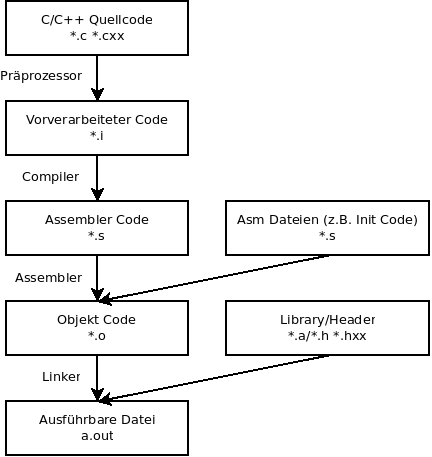
\includegraphics[width=7.5cm]{compiler}
\caption{Tool-Chain Ablauf\cite{compile}}
\label{fig:compiler}
\end{wrapfigure}

Bevor der Quellcode weiter verarbeitet wird, wird der \emph{Präprozessor} verwendet, um speziell für diesen geschriebene Makros auszuführen. Diese können verwendet werden, um zum Beispiel zu kontrollieren welcher Code kompiliert werden soll. Ein Beispiel hierzu ist in Quellcode-Listing \ref{lst:preproc} zu sehen. Hier wird überprüft ob das Präprozessor-Makro SCHALTER definiert ist und dementsprechend entschieden welcher Code aus der Datei genutzt werden soll. Die Variable SCHALTER kann nun zum Beispiel beim Compiler-Aufruf übergeben werden oder über eine Header-Datei definiert sein.

Einfache Anweisungen, wie im genannten Beispiel, könnten zwar auch in C-Code realisiert werden, jedoch besitzt die Präprozessor-Möglichkeit einen großen Vorteil. Der Quellcode wird auf die verbleibenden Zeilen gekürzt, was dem Compiler zum Beispiel bei der Optimierung die Arbeit erleichtert.

\begin{lstlisting}[frame=single, float, caption={Beispiel für Präprozessor-Anweisungen}, label={lst:preproc}]
#ifdef SCHALTER
  printf("1");
#else
  printf("2");
#endif
\end{lstlisting}

Nachdem nun die Präprozessor-Makros verarbeitet wurden, folgt der nächste Schritt. Während des \emph{Kompilierens} wird der C-Quellcode in Assembler-Code umgewandelt. Innerhalb dieses Schritts können verschiedene \emph{Optimierungen} durchgeführt werden. So kann durch den Compiler erkannt werden, ob bestimmte Variablen überhaupt benötigt werden. Auch die Verwendung der internen, schnellen Register wird in dieser Phase festgelegt. Hierdurch können unnötige, langsame Speicher-Zugriffe vermieden, und die Ausführung beschleunigt werden.

Um nun den entstandenen Assembler-Code in tatsächlichen Maschinen-Code umzuwandeln, wird der \emph{Assembler} verwendet. Dessen Aufgabe ist es lediglich die Assembler-Befehle in die dazugehörigen Opcodes umzuwandeln. Diese werden dann in Objekt-Dateien gespeichert.

Bis hierher wurde jede Quellcode-Datei einzeln behandelt. Doch um ein Programm komplett fertig zu stellen, müssen nun die verschiedenen Objekt-Dateien zu einer einzigen Datei zusammengeführt werden. Diese Aufgabe erfüllt der \emph{Linker}. Dieses Programm liest ein sogenanntes Linker-Skript und entscheidet daraufhin welche Programmteile an welche Stelle in der endgültigen Datei stehen sollen. Hierüber können auch die unterschiedlichen Speicher-Bereiche eines Embedded-Systems verwaltet werden. Der Linker kann verschiedene Ausgabe-Dateien produzieren. Eine bin-Datei beinhaltet zum Beispiel das Programm im Binär-Format als kompletten Speicherabdruck. Eine elf-Datei hingegen besitzt eine Struktur und kann zusätzliche Informationen beinhalten. Um die Ausgabedatei möglichst klein zu halten, werden in diesem Schritt alle nicht benötigten Variablen und Funktionen entfernt.

Nachdem der Quellcode nun durch alle vier Phasen bearbeitet wurde, ist das endgültige Programm fertig.

Die verschiedenen Schritte der Tool-Chain, sind auf heutigen Systemen meist nicht mehr getrennt sichtbar. So existiert zwar in der GNU Compiler Collection das Programm \emph{gcc} als Compiler, \emph{gas} als Assembler und \emph{ld} als Linker, jedoch werden die Programme meist implizit aufgerufen.

Da spätestens beim Assembler hardwareabhängige Entscheidungen getroffen werden, existieren Einschränkungen. So müssen für verschiedene Plattformen auch unterschiedliche Compiler verwendet werden. Die GNU Compiler Collection bietet hier die Möglichkeit die Zielplattform beim Kompilieren zu übergeben.


\section{Speichermodell}
\label{sec:speichermodel}

\begin{wrapfigure}{R}{0.5\textwidth}

\includegraphics[width=7.5cm]{MemoryMap}
\caption{Speichermodell-Aufbau}
\label{fig:speichermodel}
\end{wrapfigure}

Um innerhalb eines Embedded-Systems auf die einzelnen Hardware-Bausteine, wie Timer oder ähnliches, zuzugreifen werden die entsprechenden Register über einen gesamten Speicherbereich verwaltet. So verwendet ein 32-Bit ARM Prozessor einen Speicherbereich, der über 32-Bit Adressen angesprochen wird. Jedoch sind natürlich nicht alle Speicher-Bereiche vergeben. Eine grobe Aufteilung vom Speicher bei der verwendeten Plattform ist in Abbildung \ref{fig:speichermodel} zu sehen.

In den Bereichen \emph{Internal} und \emph{External RAM/ROM} sind die entsprechenden Speicher-Bereiche untergebracht. Der an Adresse null liegende Bereich kann entweder den \emph{externen ROM} oder den \emph{internen RAM} darstellen. Dies wird verwendet, um die \emph{Interrupt-Vektor-Tabelle} an dieser Adresse halten zu können. Hinter den Bereichen \emph{Miscellaneous} verbergen sich weitere Speicher-Bereiche die in diesem Projekt nicht verwendet werden, wie zum Beispiel die USB-Ports. Der Bereich \emph{Peripherals} stellt die internen Bausteine des Prozessors dar. Diese sind im Datenblatt\cite{manualat91rm9200} nachzulesen.



\section{Debug-Möglichkeiten}
\label{sec:debug}
% Wie kann man bei Embedded Systemen Debuggen
Die Möglichkeiten zum \emph{Debuggen} bei Embedded-Plattformen unterscheiden sich stark von denen bei der üblichen Programmierung. In diesem Kapitel werden einige Verfahren erläutert, mit denen während dieser Arbeit, Fehler im Quellcode gefunden wurden.

Vor allem zu Beginn eines Projekts ist der ausgeführte Quellcode relativ übersichtlich und kurz. Während dieser Zeit kann mit Hilfe des \emph{gdb} jeder \emph{einzelne Schritt} überprüft und nachvollzogen werden. Dies ist vor allem bei der Low-Level-Initialisierung in Assembler hilfreich. Sobald jedoch der erste Teil korrekt ausgeführt wird, kann das einzelne Durchgehen des Quellcodes sehr Zeitaufwändig werden. An dieser Stelle ist es hilfreich die \emph{Breakpoints} zu verwenden. Diese stoppen die Ausführung, sobald eine vorher angegebene Speicher-Adresse angesprungen wird. Da jedoch nicht immer klar ist in welchen Funktionen Fehler auftreten, können \emph{Endlos-Schleifen} hilfreich sein. Diese können an verdächtige Stellen im Code eingetragen werden und sobald die Ausführung des Codes an einer dieser Schleifen stehen bleibt, kann der Code-Bereich genauer betrachtet werden.

Es ist offensichtlich, dass die bisherigen Möglichkeiten sehr unpraktisch sind. Da zu Beginn der Portierung jedoch keine Ausgabe-Ports oder ähnliches zur Verfügung stehen, ist dies bereits eine gute Möglichkeit. Nachdem jedoch LEDs und eine serielle Schnittstelle eingerichtet sind, bestehen weitaus bessere Methoden. So können \emph{LEDs} an bestimmten Stellen ein- und ausgeschaltet, oder Daten und Meldungen über die \emph{serielle Schnittstelle} ausgegeben werden.

Sobald das Betriebssystem rudimentär läuft erhalten wir weitere Möglichkeiten. eCos bietet sowohl \emph{Tracing} als auch \emph{Assertions}. Bei aktiviertem Tracing gibt eCos bei Aufruf und return einer Funktion eine Meldung aus, sodass fehlerhafte Funktionen direkt erkannt werden können. Die sogenannten Assertions sind Prüfungen von Variablen zur Laufzeit. Hierzu werden im Quellcode Variablen und Wertebereiche angegeben, die später geprüft werden. So können fehlerhafte Funktionsaufrufe und Rückgabe-Parameter entdeckt werden.



\section{Anforderungen eines Betriebssystems an die Hardware}
\label{sec:anforderungen}
Um ein Betriebssystem auf einer Plattform ausführen zu können, werden einige \emph{hardwareabhängige Informationen} und \emph{Funktionen} benötigt. Diese werden meist über einen \emph{Hardware-Abstraction-Layer} oder einem ähnlichen Konzept zur Verfügung gestellt. Einige Betriebssysteme benötigen zudem einen Prozessor mit \emph{Memory-Management-Unit}.

Alle Scheduler, die das Unterbrechen von Tasks unterstützen (\emph{Preemption}), benötigen einen \emph{Timer} der einen \emph{Interrupt} auslöst. Hierzu müssen Funktionen definiert werden, die den Timer und Interrupt initialisieren, und Funktionen die später durch den Interrupt aufgerufen werden. Viele Plattformen besitzen einen Timer der speziell für Betriebssysteme ausgelegt ist. Der \emph{AT91RM9200} besitzt für diesen Zweck einen \emph{Periodic-Interval-Timer}, kurz PIT.

Neben den Konfigurations-Funktionen benötigt ein Betriebssystem direkt Zugriff auf die Register beim \emph{Thread-Wechsel}. Hierzu muss der bestehende Zustand aller Register gesichert und später wiederhergestellt werden. Für diesen Zweck definiert eCos verschiedene Präprozessor-Makros mit entsprechendem Assembler Code.

Neben diesen notwendigen Funktionen, müssen bei Bedarf Informationen und Funktionen zum Cache, oder anderen Hardware-Bausteinen gegeben werden.









%%%%%%%%%%%%%%%%%%%%%%%%%%%%%%% Vergleich RTOS %%%%%%%%%%%%%%%%%%%%%%%%%%%%%%%%%%
\chapter{Vergleich einiger Echtzeit-Betriebssysteme und Allgemeiner Anforderungen}
\label{sec:VergleichRTOS}
% Warum hab ich mich für eCos entschieden
% FreeRTOS, Linux RT
Bei der Auswahl eines \emph{Echtzeit-Betriebssystems}, kurz \emph{RTOS} für \emph{Realtime-Operation-System}, gibt es eine Menge Anforderungen die beachtet werden sollten. In diesem Kapitel werden zuerst \emph{allgemeine Anforderungen} näher betrachtet. Anschließend werden einige RTOS näher untersucht. Da es sich bei dieser Arbeit nicht um eine Evaluation verschiedener Betriebssysteme handelt, basieren die Ergebnisse lediglich auf meiner Recherche und nicht auf selbst durchgeführten Tests.

\section{Allgemeine Anforderungen an ein RTOS}
\label{sec:AllgemeineAnforderungen}
Im Bereich der Embedded-Entwicklung stellt sich bei der Betriebssystem-Auswahl zuerst eine Frage: Selbst ein OS entwickeln oder ein bestehendes verwenden? Die erste Möglichkeit besitzt den großen Vorteil, dass das System genau an die Bedürfnisse angepasst werden kann und keine Einarbeitung in ein großes Projekt notwendig ist. Jedoch besteht hierbei das Problem, dass keinerlei Support oder Erfahrungswerte zum System vorhanden sind.

Wenn ein bereits bestehendes Projekt verwendet werden soll, stellt sich einem Entwickler die nächste Frage: Soll ein \emph{Open-Source} Projekt verwendet werden, oder ein \emph{proprietäres}? Die Vor- und Nachteile dieser Frage sind offensichtlich. Ein Open-Source-System ist im Normalfall kostenfrei erhältlich und besitzt oft eine große Community die bei Fragen gerne hilft. Im Gegensatz dazu kostet ein Closed-Source Projekt zwar Geld, bietet jedoch professionellen Support. Auch bezüglich der Lernkurve existieren Unterschiede zwischen den beiden Möglichkeiten. Während bei proprietären Projekten die Einarbeitung durch Unterstützung des Herstellers eher leicht ist, besteht bei Open-Source Projekten oft ein Problem während der ersten Phase der Entwicklung.

Ein wichtiger Diskussions-Punkt betrifft die Open-Source Lizenz der entsprechenden Projekte. Vor allem die oft verwendete \emph{GPL-Lizenz} führt dazu, dass der Quellcode des Ziel-Projekts zur Verfügung gestellt werden muss. Dies umgehen einige Projekte, wie eCos, durch eine Zusatz-Klausel die das Linken mit GPL-Quellcode erlaubt, ohne den eigenen Quellcode veröffentlichen zu müssen.

Neben diesen offensichtlichen Möglichkeiten, bestehen einige \emph{Anforderungen}\cite{rtos_choose}, die bei der Auswahl eines Betriebssystems zu beachten sind.

\begin{itemize}
	\item Wartbarkeit/Portabilität: Dieser Punkt betrifft eigentlich alle Systeme. Eine gute Portabilität ist vor allem bei Systemen wichtig, die lange Zeit im Einsatz bleiben sollen, und eventuell auf neuere Hardware portiert werden muss.

	\item Geschwindigkeit: Geschwindigkeit ist gerade bei Zeitkritischen und Rechenintensiven Systemen ein wichtiger Punkt. Da es sich hierbei jedoch nur um die Geschwindigkeit des Betriebssystems bei Thread-Wechseln und ähnlichem handelt, ist dieser Punkt für die meisten System vernachlässigbar.

	\item Determinierbarkeit: Bei Echtzeit-Systemen kommt es auf eine zuverlässige Zusicherung der Zeitgrenzen an. Hiermit ist der Zeitunterschied zwischen dem Best-Case und dem Worst-Case gemeint. Eine große Differenz zwischen diesen Zeiten kann zu einem schwer definierbaren Zeitverhalten führen.

	\item Zuverlässigkeit: Vor allem bei Embedded-Systemen, bei denen spätere Patches nicht mehr möglich sind, ist Zuverlässigkeit ein Kernaspekt. Aber auch in Bezug auf des Entwicklungs-Modell kann dies einen Einfluss haben. So existieren viele Open-Source Projekte ohne einen festen Release-Zyklus, was unter Umständen zu veralteter Software führen kann.

	\item Skalierbarkeit/Konfigurierbarkeit: Diese beiden Punkte betreffen sowohl Hardware als auch Software. Im Bezug auf das Betriebssystem handelt es sich hierbei vor allem um die Möglichkeit neue Funktionen oder Programmteile hinzuzufügen.

	\item Ressourcenbedarf: Da in Embedded-Geräten oft nur stark begrenzter Speicherplatz vorhanden ist, muss die Größe des Betriebssystems an die Hardware angepasst werden.

	\item Kosten: Bei proprietären Projekten zählen vor allem die Lizenzkosten. Außerdem sollten hier die Entwicklungskosten mit eingerechnet werden. Diese sind eventuell bei Open-Source Projekten, durch fehlerhafte Programmteile oder eine längere Einarbeitungszeit, höher.

	\item Zertifizierbarkeit: In vielen Bereich in denen es um Sicherheit oder ähnlich kritische Aspekte geht müssen bestimmte Zertifizierungen erreicht werden. 

\end{itemize}



\section{Vergleich einiger Echtzeit-Betriebssysteme}
\label{sec:VergleichRTOS}
% WinCE, Linux
% QNX, VxWorks
% eCos, FreeRTOS
Nachdem im vorherigen Kapitel die wichtigsten Anforderungen genannt wurden, sollen nun einige \emph{Echtzeit-Betriebssysteme} verglichen werden. Hierzu werden Systeme aus drei Gruppen betrachtet. Zum einen die vom klassischen PC stammenden System \emph{Windows Embedded CE} und \emph{Linux}. Zweitens, die proprietären Systeme \emph{QNX} und \emph{VxWorks}. Und zum Schluss die beiden Open-Source Projekte \emph{eCos} und \emph{FreeRTOS}. Neben diesen ausgewählten Betriebssystemen existiert noch eine Reihe weiterer, stark verbreiteter Echtzeit-Betriebssysteme. Da jedoch zu Beginn dieses Projekts die Wahl zwischen FreeRTOS und eCos stand, sollen hier nur ein paar mögliche Alternativen betrachtet werden.

Zwar haben \emph{Windows CE} und \emph{Linux} ihre Wurzeln beim klassischen Desktop-PC oder Server, jedoch ist es auch möglich diese im Embedded- und Echtzeit-Bereich zu verwenden. So ähnelt Windows CE zwar im Aufbau und in der Bedienung den Desktop-Versionen, jedoch besitzt es einen neu entwickelten Kernel, der auch Echtzeit-Bedingungen erfüllt. Um Linux als RTOS zu verwenden, muss ein wenig mehr Arbeit in das Projekt gesteckt werden. Hier gibt es eine Reihe verschiedener Ansätze, wie RTLinux, das Real Time Application Interface oder einen RT-Patch für den Kernel. 

Sowohl Windows als auch Linux besitzen jedoch eine Schwäche: sie basieren auf ihren PC-Varianten. Dies führt dazu, dass die Systeme einigen Ballast, und somit Hardware-Voraussetzungen mitbringen. Beide Systeme sind auf den Betrieb mit Memory-Management-Unit ausgelegt und können nicht ohne diese funktionieren.

Ein weiterer Nachteil ist der relativ hohe Speicher-Verbrauch beider Systeme. So beträgt die Größe des Linux-Kernels alleine schon mindestens etwa 2 MByte. Und um die vollen Möglichkeiten von Windows CE auszunutzen ist oft das .NET-Framework notwendig, was schnell zu Größen im Bereich von 10 MByte führen kann. Im Gegensatz dazu können reine Echtzeit-Betriebssysteme Größen unter einem MByte erreichen. 

Da Ziel dieses Projekts ein \emph{POSIX-kompatibles} System ist, scheidet Windows CE aus. Diese Eigenschaft würde Linux zwar bieten, jedoch ist der Umfang der Funktionen und Möglichkeiten bei weitem nicht notwendig, wodurch auch Linux ausscheidet.

Die nächsten beiden Betriebssysteme die betrachtet werden, sind \emph{QNX} und \emph{VxWorks}. Beide Systeme sind auf den Echtzeit-Betrieb optimiert und werden bereits seit über 25 Jahren entwickelt. Während VxWorks einen monolithischen Kernel verwendet, arbeitet in QNX ein Mikro-Kernel. Vor allem QNX ist ein sehr umfangreiches System. Es benötigt ähnlich wie Linux eine MMU, besitzt zusätzlich eine grafische Oberfläche und kann einen Paket-Manager verwenden. Da sowohl VxWorks, als auch QNX proprietäre Lizenzen verwenden, in diesem Projekt jedoch möglichst freie Software verwendet werden soll, scheiden auch diese beiden als mögliche Systeme aus.

Drei der bisher beschriebenen Systeme, namentlich \emph{Windows}, \emph{Linux} und \emph{QNX}, sind sogenannte \emph{Self-Hosting} Betriebssysteme. Bei diesen ist es im Betrieb möglich das System zu verändern. Dies besitzt den Nachteil, dass ein Dateisystem nötig ist und so unter Umständen die Echtzeit-Fähigkeit beeinflusst wird. Vor allem wird jedoch die Komplexität des Systems erhöht, was zu einem schlechteren Überblick bei der Entwicklung und Portierung führt. Bei den anderen drei Systemen müssen alle Einstellungen zur Compile-Zeit vorliegen. Das besitzt den Vorteil, dass während des Linkens alle unnötigen Funktionen entfernt werden können und so die Größe möglichst gering gehalten wird.

Die zwei verbleibenden Echtzeit-Betriebssysteme sind \emph{eCos} und \emph{FreeRTOS}. Sie stehen beide unter einer modifizierten GPL-Lizenz und besitzen eine ähnliche Funktionalität. Beide bieten POSIX-Unterstützung, Unterstützung für viele verschiedene Hardware-Architekturen und die üblichen Synchronisations-Mechanismen wie Mutexe und Semaphoren. Außerdem bietet eCos $\mu$ITRON Kompatibilität. Von FreeRTOS besteht zudem ein Neben-Projekt, namens SafeRTOS. Dieses basiert auf dem FreeRTOS Quellcode und wurde zusätzlich nach IEC 61508 zertifiziert, was die Verwendung in sicherheitskritischen Bereichen ermöglicht.

Für dieses Projekt wurde trotz der ähnlichen Eigenschaften \emph{eCos} ausgewählt. Diese Entscheidung basiert auf drei Punkten. Zum Ersten besitzt eCos bereits in der Standard-Distribution einen \emph{IPv6-Stack}, der für weitere Projekte nötig ist. Dieser Stack basiert auf dem FreeBSD TCP/IP Stack von 2001. Eine oft angeführte Kritik ist das Alter dieses Pakets was zu einigen bekannten Bugs führt. Jedoch besitzt FreeRTOS keinen direkt IPv6 Support. Zweiter Auswahl-Grund ist die sehr ausführliche \emph{Dokumentation} von eCos. Und letzter Grund ist der Bootmanager \emph{RedBoot}. Dieser verwendet den Hardware-Abstraction-Layer von eCos und ermöglicht in Zukunft auch Projekte die auf Linux basieren.








%%%%%%%%%%%%%%%%%%%%%%%%%%%%%%% Verwendete Hard- und Software %%%%%%%%%%%%%%%%%%%%%%%%%%%%%%%%%%
\chapter{Verwendete Hard- und Software}
\label{sec:HardSoftware}
% UNC90, AT91RM9200...
% Ubuntu, OpenOCD 0.4.0...
Dieses Kapitel enthält eine Erläuterung der verwendeten Hardware und Software.


\section{Hardware}
\label{sec:hardware}
Die verwendete ARM-Plattform besteht aus einem \emph{Digi UNCBAS3} Entwicklungsboard. Auf diesem sitzt ein \emph{UNC90} Prozessormodul mit einem \emph{Atmel AT91RM9200} Prozessor. Im folgenden werden die einzelnen Komponenten und deren Eigenschaften näher erläutert.

Das \emph{UNCAS3} Entwicklungsboard von Digi (ehemals FS Forth) enthält ein Slot für ein \emph{UNC20} oder \emph{UNC90} Prozessormodul. Des weiteren stellt es eine Reihe von Anschlüssen zur Verfügung.

\begin{itemize}
	\item Ethernet Schnittstelle
	\item Serielle Schnittstelle
	\item Parallele Schnittstelle
	\item 20 Pin JTAG Interface
	\item Jeweils 2 LEDs und Taster, sowie ein Reset-Taster
	\item Interface für externes Charakter Display
	\item USB Host und Device Unterstützung
\end{itemize}

Das verwendete \emph{UNC90} Prozessormodul integriert neben dem Prozessor insgesamt 16 MByte SDRAM und Flash. Außerdem enthält es einen Ethernet PHY und unterstützt alle vom Board bereitgestellten Schnittstellen.

Ein \emph{Atmel AT91RM9200} Prozessor arbeitet als Kernstück auf dem UNC90. Dieser Prozessor basiert auf einem ARM920T Design und taktet mit maximal 180 MHz. Er besitzt eine Memory-Management-Unit und einen Instruction- sowie Data-Cache. Außerdem sind 16 kByte SRAM und 128 kByte ROM verbaut. Zusätzlich werden diverse Schnittstellen zum Verwenden von externen RAM, ROM und anderen Dingen zur Verfügung gestellt.

\begin{itemize}
	\item External Bus Interface zur Anbindung von externem Speicher
	\item Ethernet Interface
	\item USB 2.0
	\item Multimedia Card Interface
	\item 4 USART
	\item Serial Peripheal Interface
	\item Two Wire Interface
\end{itemize}

Um eine JTAG-Verbindung per USB herzustellen, wird ein \emph{Olimex ARM-USB-OCD} Debugger verwendet. Dieser stellt außerdem eine serielle Schnittstelle und kann als Spannungsversorgung per USB dienen. Letzteres wird in diesem Projekt nicht verwendet.





\section{Software}
\label{sec:Software}
Die Arbeit an eCos fand an einem \emph{GNU/Linux} System statt. Um eCos und damit \emph{GNU Make} und die \emph{GNU Compiler Collection} zu verwenden, wird ein POSIX-kompatibles System benötigt. Somit ist das Arbeiten unter Windows nur mit Hilfe von Kompatibilitäts-Schichten wie \emph{Cygwin} möglich. Um eine spätere Nachvollziehbarkeit herzustellen, werden im Folgenden die verwendeten Anwendungen und Versionen erläutert. Alle nicht gelisteten Pakete wurden aus den offiziellen Ubuntu Repositories\footnote{Einzusehen unter \url{packages.ubuntu.com}} installiert.

Als Betriebssystem wird eine 32-bit Version von \emph{Ubuntu 10.10} Maverick Meerkat verwendet. Diese integriert einen \emph{2.6.35 Linux Kernel}. Zur Erleichterung des Bau-Prozesses wird \emph{GNU Make 3.81} verwendet. \emph{OpenOCD} ist in der Version 0.4.0 installiert. Dies ist das aktuellste stabile Release.

Die Anwendungen der \emph{GNU ARM Toolchain} wurden als Binarys in der Version 3.4 heruntergeladen\footnote{Quelle: \url{www.gnuarm.com}}. Dies Paket enthält folgende Bestandteile:
\begin{itemize}
	\item GNU Binutils 2.15
	\item GNU Compiler Collection gcc 3.4.4 mit Unterstützung für C, C++ und Java
	\item Newlib 1.12.0
	\item Insight 6.1
\end{itemize}

Der Quellcode von \emph{eCos} wurde mit Hilfe eines Installations-Tools in der Version 3 heruntergeladen. Dies enthält außerdem Binaries der Konfigurations-Anwendungen.










%%%%%%%%%%%%%%%%%%%%%%%%%%%%%%% eCos Allgemein %%%%%%%%%%%%%%%%%%%%%%%%%%%%%%%%%%
\chapter{eCos Allgemein}
\label{sec:eCos}
% Wie ist eCos aufgebaut
Das Echtzeit-Betriebssystem eCos, der Name steht für \emph{embedded configurable operating system}, wurde zunächst von Cygnus Solutions entwickelt. Diese Firma wurde später von Red Hat übernommen, die die Entwicklung von eCos weitgehend eingestellt hat. Während dieser Zeit wurde das Betriebssystem jedoch von den ehemaligen Mitarbeitern weiterentwickelt. Im Januar 2004 übergab Red Hat, auf Anfrage der eCos Entwickler, die Rechte an die Free Software Foundation. Diese stellte den Quellcode unter der \emph{GNU Public License} frei zur Verfügung. Außerdem fügten sie der Lizenz eine Ausnahme hinzu, die erlaubt beliebige Software gegen eCos zu linken, ohne die eigene Software auch unter die GPL stellen zu müssen. Mit dieser Ausnahme entspricht die Lizenz in etwa der \emph{LGPLv3}. Dies wird benötigt, da der eCos Kernel selbst separat kompiliert wird, und der Code der eigenen Applikation gegen diesen gelinkt wird.

Die relativ starke Verbreitung von eCos hat dazu geführt, dass eine Vielzahl an Plattformen unterstützt werden. Darunter sind zum Beispiel typische Embedded Architekturen wie \emph{ARM}, \emph{MIPS}, \emph{Motorola 68k} und \emph{NIOS II}, jedoch auch Architekturen wie \emph{Intel x86}, \emph{IA-32}, \emph{PowerPC} oder \emph{SPARC}. Es existieren sogar Portierungen für die Sega Spielekonsole \emph{Dreamcast}, und die Virtualisierungs-Software \emph{VMware}.

Im weiteren dieses Kapitels werden einige wichtige Informationen zum Aufbau von eCos gegeben.

\section{Konfigurierbarkeit von eCos}
\label{sec:config}
% Wie funktioniert das konfigurerien
% CDL
Eine Stärke von eCos ist die gute Konfigurierbarkeit. Hierzu wird ein eigenes Paketsystem und Konfigurationstool verwendet. Somit ist es möglich ein System auf genaue Anforderungen anzupassen. Kernstücke dieses Konfigurationssystems sind das \emph{Konfigurationstool}, die \emph{eCos Datenbank} und die \emph{CDL Skript-Sprache}.

\emph{CDL} steht für Component Definition Language und ist eine Skript-Sprache, die speziell zum Beschreiben von Konfigurationen und ähnlichem entwickelt wurde. Innerhalb von eCos wird sie verwendet, um die Eigenschaften der Pakete zu beschreiben. Hierzu enthält jedes Paket eine dazugehörige cdl-Datei, die die verfügbaren Option angibt. In dem Quellcode-Listing \ref{lst:cdl_baud} ist eine mögliche Option für einen Treiber einer seriellen Schnittstelle zu sehen. Neben einfachen Option ist es auch möglich Werte berechnen zu lassen. Außerdem existieren eine Reihe weiterer Befehle, um Angaben über ein Paket zu machen. So könnte ein Paket eine bestehende Schnittstelle implementieren oder aber ein anderes Paket benötigen. Die weiteren Details dieser Sprache sollen hier nicht erläutert werden, da dies den Rahmen dieser Arbeit sprengen würde. Außerdem wurde dieser Teil von eCos kaum bearbeitet.

\begin{lstlisting}[frame=single, float, caption={CDL Option zum Setzen der Baud Rate}, label={lst:cdl_baud}]
cdl_option CYGDBG_SERIAL_BAUD {
	display          "Set Baud Rate"
	flavor           data
	default_value    38400
	description      "
	    Set baud rate of serial console"
}
\end{lstlisting}

% eCos DB
Die Datei \texttt{ecos.db} enthält die sogenannte Paket-Datenbank. Dies ist eine Auflistung aller verfügbaren Pakete inklusive der entsprechenden Pfade und CDL-Skripte. Zusätzlich können hier Vorlagen, genannt \emph{targets}, für Plattformen definiert werden, die eine Zusammenfassung gewählter Pakete darstellen. Beim Erstellen eines neuen Pakets ist ein Eintrag in diese Datei nötig, sodass die verwendeten Konfigurations-Anwendungen eine vollständige Liste der zur Verfügung gestellten Pakete erhalten.

% Anpassen...
\begin{figure}
\centering
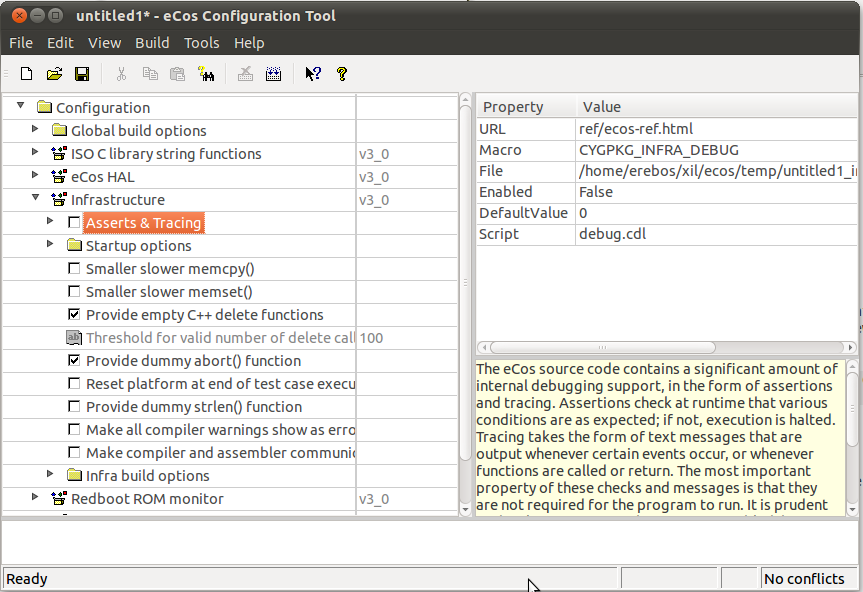
\includegraphics[width=12cm]{configtool}
\caption{eCos Configtool}
\label{fig:configtool}
\end{figure}

% Configtool mit Screenshot
Das \emph{configtool} ist ein grafisches Frontend zum Erstellen neuer eCos-Projekte. In Abbildung \ref{fig:configtool} ist ein Screenshot hiervon zu sehen. Um ein neues Projekt zu erstellen, kann ein Template verwendet werden. Hierdurch werden benötigte Pakete automatisch hinzugefügt. Es können jedoch auch Pakete von Hand hinzugefügt werden. Anschließend ist es möglich die Paket-Optionen einzustellen, um zum Beispiel die serielle Schnittstelle zu wählen. Falls das Projekt korrekt konfiguriert wurde und alle gewünschten Pakete hinzugefügt wurden, kann das Projekt gespeichert werden. Hierbei wird eine ecc-Datei angelegt, die die Projekt-Eigenschaften enthält. Diese kann später auch wieder mit dem configtool geöffnet und verändert werden. Zusätzlich wird beim Speichern ein sogenannter \emph{Build-Tree} und ein \emph{Install-Tree} angelegt. Dies sind Verzeichnisstrukturen, die benötigte Dateien enthalten. Beim Speichern werden hierzu einige Dateien aus dem eCos-Quellcode-Verzeichnis herauskopiert. 

Der \emph{Build-Tree} enthält eine Verzeichnisstruktur, wie sie auch im Quellcode-Verzeichnis verwendet wird. Hier werden also die verschiedenen Pakete unterteilt. Innerhalb dieser Verzeichnisse wird eine Struktur von Makefiles angelegt. Diese werden dynamisch beim Speichern des Projektes erzeugt, da hier die Flags für Linker und Compiler verändert werden können.

Im \emph{Install-Tree} finden sich Header-Dateien. Diese werden benötigt, um Software gegen das erstellte Projekt Linken zu können. Während das Projekt mittels \texttt{make} gebaut wird, werden zusätzlich einige Verzeichnisse im Install-Tree angelegt. Das Verzeichnis \emph{bin} enthält eventuell erstellte RedBoot Images. Die von eCos unterstützen \emph{Tests} werden im gleichnamigem Verzeichnis hinterlegt. Im Verzeichnis \emph{lib} sind die eigentlichen Ausgabedateien enthalten. Hierzu gehört zum Beispiel das \emph{Linker-Skript} und die \emph{Objekt-Datei} \texttt{libtarget.a}.



\section{Hardware Abstraction Layer}
\label{sec:HAL}
Der HAL, kurz für \emph{Hardware-Abstraction-Layer}, dient als Vermittlungs-Schicht zwischen Hardware und Software. Jegliche Hardware-Zugriffe werden von diesem Paket erledigt. Dadurch ist es möglich eCos auf eine neue Plattform zu portieren ohne einen Großteil des Quellcodes zu ersetzen. Der HAL ist in verschiedene Schichten aufgeteilt. Der \emph{Architektur-HAL} abstrahiert die CPU-Architektur und allgemeine Dinge. So existiert zum Beispiel ein HAL für die ARM Architektur. Der \emph{Variant-HAL} repräsentiert verschiedene Variationen einer Prozessor-Architektur. So existiert ein Variant-HAL für den AT91RM9200 und einer für den AT91SAM7. Diese Unterscheiden sich in den genauen Spezifikationen, basieren jedoch beide auf dem selben Grund-Design. In diesem Beispiel findet sich noch ein Spezialfall. Der Variant-HAL kann auch über mehrere Teilpakete verteilt sein. So verwenden die beiden genannten Prozessortypen den selben HAL. Jedoch wird über eine CDL-Option die genaue Variation festgelegt. Der sogenannte \emph{Plattform-HAL} repräsentiert die Eigenschaften der verwendeten Plattform. Hier können zum Beispiel externe Speicher oder Interrupt-Controller eingerichtet werden.

Neben diesen hardware-spezifischen Teilen des HALs, existiert der \emph{Common-HAL}. Dieser enthält Optionen und Funktionen die alle HALs verwenden. Außerdem existieren noch sogenannte \emph{Auxiliary-HALs}. Hierrüber können Module definiert werden, die von mehreren HALs verwendet werden können.

Auch andere Betriebssysteme verwenden das Konzept einer Hardwareabstraktionsschicht. So enthielt bis vor einiger Zeit ziemlich jede Linux-Distribution ein HAL-Paket. Mittlerweile wird dieses Paket durch andere ersetzt. Aber auch diese arbeiten nach einem ähnlichen Prinzip. Auch Windows verwendet seit einiger Zeit einen HAL um die Hardware von der Software zu trennen.

In einem späteren Kapitel wird mit Hilfe eines Beispiels, der Zusammenhang zwischen dem HAL und dem restlichen System erläutert.




\section{ROM Monitor RedBoot und die Virtuelle Vektortabelle}
\label{sec:ROM_Monitor}

\emph{RedBoot} ist ein Bootloader für Embedded-System der auf dem Hardware-Abstraction-Layer von eCos basiert. Dieser bietet die Möglichkeit Anwendungen zu laden und auszuführen. Es kann sowohl die serielle als auch die Ethernet-Schnittstelle benutzen, um Images in den Speicher zu laden. Es unterstützt sowohl eCos-Anwendungen als auch Linux Images. Zusätzlich bietet es eine Kommandozeile, mit der zum Beispiel Images verwaltet werden können, oder RedBoot konfiguriert werden kann.

Neben diesen bekannten Eigenschaften, die auch andere Bootloader wie U-Boot besitzen, enthält eCos und RedBoot eine Spezialität: Die \emph{virtuelle Vektortabelle}, kurz VVT. Dies ist eine Möglichkeit um Funktionen zwischen dem ROM Monitor und einer Anwendung zu teilen.

Die virtuellen Vektoren, sind im Prinzip eine Gruppe von Zeigern auf \emph{Service-Funktionen}. Diese liegen an einer statischen Adresse im Speicher. Diese Adresse wird sowohl an RedBoot als auch an die eCos-Anwendung vor dem kompilieren übergeben.

Der weitere Verlauf lässt sich am besten an einem Beispiel erklären. Angenommen es soll ein System entwickelt werden, dass über eine serielle Schnittstelle bedient wird. Eine Möglichkeit während der Entwicklung wäre es nun, jedem Entwickler eine Plattform zu Verfügung zu stellen, um das Projekt auf der Hardware zu testen. Mit Hilfe von RedBoot wäre es jedoch möglich, die Konsolenausgabe auf die Ethernet-Schnittstelle umzuleiten, sodass alle Entwickler diese Plattform nutzen können. Hierzu müsste auf dem System RedBoot installiert sein, und die VVT von diesem übernommen werden. In dieser existiert nun ein Funktionsaufruf um eine Ausgabe über einen \emph{Communication Channel}\footnote{Communication Channels sind abstrahierte Konsolen die eCos bereitstellt. Diese können zum Beispiel serielle oder Ethernet Schnittstellen sein.} zu machen. Innerhalb von RedBoot wird diese Ausgabe auf die Ethernet-Schnittstelle gesetzt. Nun wird der eCos-Applikation mitgeteilt, dass eine VVT bereits vorhanden ist und wo diese liegt. Daraufhin kann die Anwendung kompiliert werden und mittels RedBoot in den Speicher geladen werden. Wenn nun diese Anwendung ausgeführt wird, wird die Kontrolle über das System komplett an diese abgegeben. Wenn jedoch nun eine Ausgabe erfolgen soll, wird nicht eine eigene Funktion verwendet, sondern die über die VVT definierte Ausgabe-Funktion von RedBoot.

Über diesen Wege kann eine Applikation entwickelt werden, die lediglich den für den Produktiv-Betrieb nötigen Code enthält. Somit gibt es keine Verwendung mehr für gdb-Stubs im Anwendungs-Code. Stattdessen wird RedBoot und die virtuelle Vektortabelle verwendet.

Insgesamt existieren eine Reihe an Funktionen die auf diese Weise zugegriffen werden können. Hier sollen nur ein paar wichtige genannt werden.

\begin{itemize}
	\item Interrupt Service Routine: Hierrüber könnten Interrupts durch den ROM Monitor verarbeitet werden, während die restliche Zeit die RAM Anwendung ausgeführt wird.
	\item Communication Channel Daten: Dies entspricht dem Beispiel von oben.
	\item Reset: Hierdurch kann der System-Reset verändert werden. So könnte zum Beispiel statt einem kompletten Reset, lediglich das Anwendungs-Image durch RedBoot erneut geladen und ausgeführt werden.
	\item gdb Interrupt: Mittels der gdb-Einträge in der VVT kann die Software debugged werden, ohne einen gdb-Stub in den Code zu integrieren.
\end{itemize}








\section{Verzeichnisstruktur}
\label{sec:dir}
% Wie sind die eCos Verzeichnisse aufgebaut
% ToDo: Bild
Das eCos System-Verzeichnis besteht neben den Verzeichnissen die zum Bau der Tools notwendig sind, aus den Verzeichnissen \emph{tools} und \emph{packages}. Ersteres enthält den Source-Code und die Binaries der Konfigurations-Anwendungen. Das Verzeichnis \emph{packages} enthält die eCos Datenbank und alle enthaltenen Pakete. Die Pakete sind durch Unterverzeichnisse nach Inhalt sortiert. So enthält das Unterverzeichnis \emph{hal} alle HAL-Pakete und das Verzeichnis \emph{devs}, alle Geräte-Treiber.

Jedes Paket enthält zunächst ein Unterverzeichnis mit der Versionsnummer der eCos Distribution. Innerhalb dieses Verzeichnisses ist nun die eigentliche Paket-Struktur zu erkennen. Das Verzeichnis \emph{cdl} enthält das zum Paket gehörige CDL-Skript. Der Ordner \emph{include} enthält verwendete Header-Dateien. In \emph{misc} werden verschiedene Dinge, wie zum Beispiel eine Konfigurationsdatei, untergebracht. Das Verzeichnis \emph{src} enthält den Source-Code. Die Tests des Pakets werden im Verzeichnis \emph{tests} und eventuelle Dokumentationen im Verzeichnis \emph{doc} untergebracht.




\section{Beispiel Applikation und Infrastruktur}
\label{sec:beispiel_infra}
% Wie könnte eine eCos Aplikation aussehen und funktionieren
% Wie wird die erstellt
% Was greift auf was zu...
% eCos Schichten
In diesem Abschnitt soll das Erstellen einer einfachen Applikation mit eCos erläutert werden. Hierzu werden auch Zusammenhänge zwischen den einzelnen Paketen und der eCos Infrastruktur erläutert.

%\begin{wrapfigure}{R}{0.5\textwidth}
%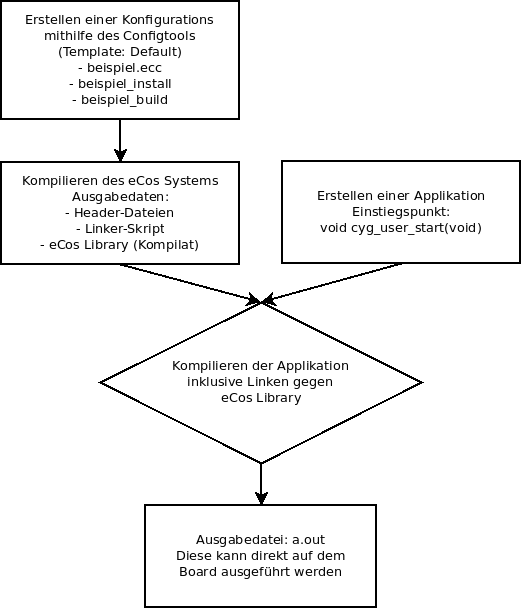
\includegraphics[width=10cm]{beispiel_flowchart}
%\caption{Flussdiagramm zum erstellen einer eCos Applikation}
%\label{fig:flowchart}
%\end{wrapfigure}

\begin{figure}
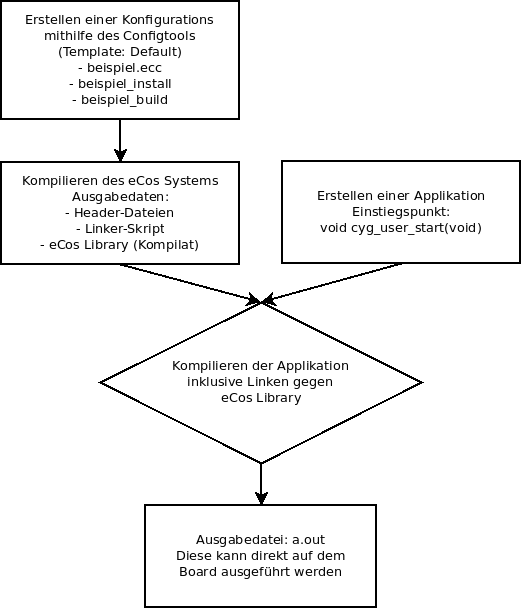
\includegraphics[width=12cm]{beispiel_flowchart}
\caption{Flussdiagramm zum Erstellen einer eCos Applikation}
\label{fig:flowchart}
\end{figure}



Das Flussdiagramm in Abbildung \ref{fig:flowchart} zeigt den Ablauf um eine eCos Applikation zu erstellen. Zu Beginn wird mit Hilfe des Configtools eine Konfiguration erstellt. Diese sollte alle benötigten Pakete, wie den HAL und den Kernel, enthalten. Hierzu können am besten die Paket-Templates verwendet werden. Die Vorlage \emph{Default} enthält die wichtigsten Pakete und dient als gute Grundlage. Beim Abspeichern der Konfiguration wird nun die gesamte Ziel-Verzeichnisstruktur erstellt. Diese besteht aus dem Install- und dem Build-Verzeichnis. Um nun den Kernel zu kompilieren, muss lediglich das \emph{Makefile} im Build-Verzeichnis ausgeführt werden. Nach einiger Zeit entsteht nun die eCos-Library, die für die weitere Entwicklung nötig ist. Diese enthält den Kernel und alle anderen, vorher ausgewählten, Pakete.

Um nun eine eigene Applikation zu erstellen, muss eine neue C-Datei erstellt werden. Da diese nicht separat ausgeführt wird, sondern durch eCos aufgerufen wird, ist der Einstiegspunkt nicht mehr die \texttt{main}-Funktion, sondern die \texttt{cyg\_user\_start}-Funktion. Wenn nun die Applikation fertig ist, kann sie gegen die eCos-Library gelinkt werden. Die daraus entstehende Ausgabe-Datei, häufig \texttt{a.out} genannt, kann nun auf das Board geladen und ausgeführt werden. Falls alles korrekt konfiguriert wurde, sollte die Applikation jetzt ausgeführt werden.

\begin{figure}
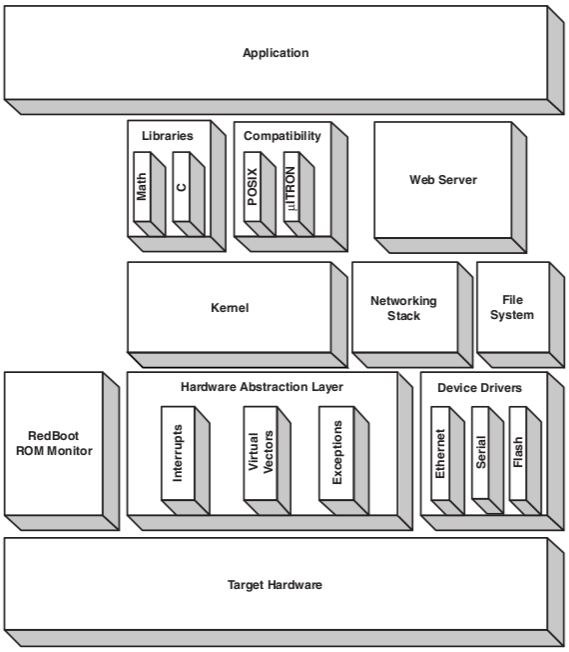
\includegraphics[width=12cm]{infra}
\caption{Infrastruktur einer eCos Applikation. Quelle:\cite{ecos_book} Seite 9}
\label{fig:infra}
\end{figure}

Jede eCos Applikation ist nach einer bestimmten Infrastruktur aufgebaut. Diese Struktur variiert je nach Paket-Zusammenstellung, entspricht jedoch immer einem bestimmten Muster. Eine möglicher Aufbau ist in Abbildung \ref{fig:infra} zu sehen.

Die Basis bildet selbstverständlich die \emph{Ziel-Hardware}. Darauf Aufbauend existieren die verschiedenen Software-Schichten von eCos. Alle Bausteine im Diagramm entsprechen einem oder mehreren Paketen. Als erste Schicht ist der \emph{Hardware-Abstraction-Layer} zu sehen. Dieser abstrahiert die Hardware, sodass die darüber liegenden Schichten plattformunabhängig arbeiten können. Auch der danebenliegende ROM Monitor \emph{RedBoot} baut auf diesen auf, was den HAL zum grundlegenden Paket macht. Um verschiedene Geräte anzusprechen, existieren eine Reihe weiterer Pakete auf der untersten Ebene. Diese \emph{Treiber} können während der Konfiguration beliebig hinzugefügt werden und stellen dementsprechend die Hardware dar. Eine Reihe von Hardware-Bausteinen wird bereits von eCos unterstützt, was die Entwicklung stark vereinfachen kann.

Auf der nächsten Ebene befindet sich der \emph{Kernel}. Dieser ist das Herzstück der Software und enthält die Grundlagen des Betriebssystems, wie den Scheduler, die Definition von Threads und Synchronisations-Mechanismen. Neben dem Kernel existieren einige weitere grundlegende Pakete. In diesem Beispiel ein \emph{Netzwerk Stack} und ein \emph{Dateisystem}. Diese Art von Paketen wird zum Beispiel bei Linux als Kernel-Module zur Verfügung gestellt. Hierdurch können darauf aufbauende Applikationen direkt auf die Funktionalität der Pakete zugreifen.

Die vierte Schicht des Diagramms repräsentiert eine \emph{Vermittlungs-Schicht} zwischen dem abstrahierten Betriebssystem und der Benutzer-Applikation. Hier sitzen zum Beispiel Pakete, die eine Kompatibilitäts-Schicht bereitstellen. In diesem Beispiel ein \emph{POSIX-} und ein \emph{$\mu$ITRON-Paket}. Aber auch die \emph{ISO-C-Library} oder die \emph{Math-Library} sind in dieser Schicht enthalten. Neben diesen Unterstützungs-Funktionen können jedoch auch Applikationen hier enthalten sein. Hierzu bietet eCos bereits einige Pakete, um zum Beispiel einen Webserver, einen VNC- oder FTP-Server aufzusetzen.

Auf der obersten Ebene des Modells ist die \emph{Benutzer-Applikation}. Diese kann direkt und indirekt auf die darunter liegenden Schichten zugreifen, und somit die volle Funktionalität dieser nutzen.






























%%%%%%%%%%%%%%%%%%%%%%%%%%%%%%% Umsetzung %%%%%%%%%%%%%%%%%%%%%%%%%%%%%%%%%%
\chapter{Umsetzung}
\label{sec:Umsetzung}
% Was hab ich wie und wann im Projekt gemacht...
% Quellcode auf CD packen...
In diesem Kapitel wird der Fortschritt des Projekts in chronologischer Reihenfolge erläutert. Hierbei werden relevante Probleme und der erstellte Code näher betrachtet. Zur besseren Übersicht werden lediglich Code-Ausschnitte beschrieben. Der gesamte Quellcode ist auf der beigelegten CD enthalten.



% Konfiguration OpenOCD, gdb...
% Aufbau des Boards (USB an PC, JTAG an Board...)
\section{Vorbereitung durch Praxis-Projekt}
\label{sec:Vorbereitung}
Die Aufgabe innerhalb meines Praxis-Projekts bestand in dem Zusammenstellen einer \emph{Tool-Chain} für die genannte ARM-Plattform. Hierzu wurde auch ein Basis-Programm, zum Erstellen von beliebigen Anwendungen für das Board, erstellt. Der hierin verwendete Code dient als Grundlage, für das Portieren von eCos. Hierbei ist vor allem der \emph{Startup-Code} und die \emph{Konfiguration} des OpenOCD hilfreich.

% evtl. Bild vom Aufbau hinzufügen???
Um mit dem Board zu kommunizieren, werden vor allem die JTAG- und die serielle Schnittstelle verwendet. Diese werden beide an den \emph{Olimex ARM-USB-OCD Debugger Adapter} angeschlossen. Dieser wird verwendet, um die beiden Signale mittels USB ansprechen zu können. Dadurch wird die serielle Schnittstelle über USB direkt als Gerät erkannt, und kann unter Linux als \emph{/dev/ttyUSB0} angesprochen werden. Zusätzlich kann der Adapter die Geschwindigkeit der JTAG-Schnittstelle erhöhen. Bei einem direkten Anschluss des PCs an die JTAG-Schnittstelle mittels des Parallel-Ports muss der Host jede Bitänderung von Hand realisieren. Dies führt zu einer hohen CPU Belastung, welche vom Adapter übernommen wird. Außerdem können einige Aufgaben, wie das ständige Abfragen eines Zustands, vom JTAG-Adapter übernommen werden.

Um die JTAG-Schnittstelle anzusprechen, wird auf Host-Seite der \emph{Open On Chip Debugger}, kurz OpenOCD, verwendet. Dieses Open Source Projekt wurde im Rahmen einer Diplom-Arbeit an der Universität Augsburg geschaffen, und erfreut sich seitdem großer Beliebtheit. Es stellt eine Client-Server-Architektur zur Verfügung, mit der die Hardware angesprochen werden kann. Hierzu wird ein OpenOCD-Server gestartet, auf den mit \emph{Telnet} zugegriffen werden kann. Falls gewünscht kann auch ein \emph{gdb-Server} dazu gestartet werden, der die Anfragen direkt an den OpenOCD Server weiter gibt. Auf diese Konfiguration kann mit Hilfe vom \texttt{gdb} und falls erwünscht einem Frontend zugegriffen werden. Anschließend kann der \texttt{gdb} wie gewohnt bedient werden und mit voranstellen des Schlüsselwortes \texttt{monitor} auf die OpenOCD-Funktionen zugegriffen werden.

\begin{lstlisting}[frame=single, float, caption={OpenOCD Konfiguration}, label={lst:openocd_config}]
interface ft2232
ft2232_device_desc "Olimex OpenOCD JTAG"
ft2232_layout olimex-jtag
ft2232_vid_pid 0x15ba 0x0003

reset_config trst_and_srst

jtag newtap at91rm9200 cpu -irlen 4 -ircapture 0x1 -irmask 0xf -expected-id 0x05b0203f
target create at91rm9200.cpu arm920t -endian little -chain-position at91rm9200.cpu

at91rm9200.cpu configure -work-area-virt 0x00200000 -work-area-phys 0x00200000 -work-area-size 0x4000 -work-area-backup 1

flash bank cfi 0x10000000 0x1000000 2 2 at91rm9200.cpu
\end{lstlisting}

Damit dem OpenOCD die Struktur der Hardware bekannt ist, muss ihm eine \emph{Konfigurationsdatei} übergeben werden. Das Quellcode-Listing \ref{lst:openocd_config} enthält eine vereinfachte Version der verwendeten Konfiguration. In den ersten vier Zeilen wird der \emph{JTAG-Adapter} beschrieben. Hierzu enthält der OpenOCD bereits einige Layouts, sodass diese einfach verwendet werden können. Zeile sechs definiert das \emph{Reset Verhalten}. In diesem Fall sollen sowohl das System, als auch die Test-Logik zurückgesetzt werden. In den Zeilen acht und neun wird ein Ziel für die JTAG-Schnittstelle eingerichtet und anschließend ein gdb-Ziel eingerichtet und damit der gdb-Server gestartet. Dies ist notwendig, da JTAG mehrere Test-Logiken (genannt TAPs) und Module im Ziel unterstützt. Diese können zum Beispiel in Reihe gesetzt und einzeln angesprochen werden. Die zweitletzte Zeile richtet einen \emph{Arbeitsbereich} für den Debugger im internen RAM ein. Dies wird verwendet, um das laden eines Image zu beschleunigen. Die letzte Code-Zeile richtet den \emph{externen Flash} für den Debugger ein. Seit einem OpenOCD Update auf Version 0.4.0 hat sich die Syntax dieses Befehls geändert, sodass der Flash nicht eingerichtet wird. Da der Flash in diesem Projekt nicht verwendet wird, soll er an dieser Stelle auch nicht weiter beachtet werden.

% Openocd Skript und load befehle
\begin{lstlisting}[frame=single, float, caption={OpenOCD Kommandos zum starten eines Programms}, label={lst:openocd_startup}]
monitor reset halt
monitor script [Script]
monitor load_image [Bin-File]
monitor reg pc [Adresse]
monitor resume
\end{lstlisting}

Um nun eine Binär-Datei in den Speicher zu laden, und diese auszuführen, müssen die in Listing \ref{lst:openocd_startup} zu sehenden Kommandos ausgeführt werden. Zuerst muss die Hardware zurückgesetzt werden. Anschließend wird ein Skript zur \emph{Initialisierung} ausgeführt. Dieses wird später noch genauer betrachtet. In Zeile drei wird nun die Binär-Datei in den Speicher geladen. Wenn es sich dabei um eine ELF-Datei oder eine andere formatierte Datei handelt, werden die Speicher-Bereiche automatisch erkannt. Andernfalls muss die Ziel-Adresse von Hand angegeben werden. Falls der Start des Programms sich nicht an Adresse null befindet, kann der \emph{Program-Counter} mittels des Befehls in Zeile vier gesetzt werden. Anschließend kann mittels \texttt{resume} das Programm ausgeführt werden. Für den Fall, dass das Programm in einen Flash geladen werden soll, muss anders vorgegangen werden.

\begin{lstlisting}[frame=single, float, caption={OpenOCD Skript zum Initialisieren der Hardware}, label={lst:openocd_skript}]
# mww := Memory Write Word
# Enable Main Oscilator 
mww 0xfffffc20 0x0000ff01
[...]
mww 0xfffff870 0xffff0000
mww 0xfffff874 0x00000000
[...]
# Remap um internen RAM an Adresse 0x0 zu setzen
mww 0xffffff00 0x00000001
\end{lstlisting}

Ein Auszug aus dem Inhalt des in Zeile zwei ausgeführten \emph{Skripts} ist in Listing \ref{lst:openocd_skript} zu sehen. Dieses initialisiert die Hardware, sodass der Debugger zum Beispiel auf den externen RAM zugreifen kann. Da dieser erst konfiguriert werden muss und zusätzlich von der System-Clock abhängt muss dies vor dem Laden der Binär-Datei geschehen. Wie im Quellcode zu sehen ist, besteht das Skript aus Befehlen für den OpenOCD. Da diese relativ unleserlich sind, und lediglich spezielle Speicher-Adressen beschreiben, werden ich nicht weiter auf den Inhalt eingehen.



% Einarbeitung
% HAL einrichten und CDL
% Startup Code; var_io.h
\section{Einarbeitung und erste Ansätze}
\label{sec:Einarbeitung}
Der erste Ansatz des Portierens orientiert sich an dem \emph{Porting Guide} der eCos Referenz\cite{ecos_ref}. Hierzu wird ein bestehendes HAL-Paket als Basis genutzt und an die eigene Plattform angepasst. Als Grundlage habe ich hierzu den HAL des \emph{AT91SAM7} verwendet. Dieser Prozessor ähnelt dem \emph{AT91RM9200} stark, sodass große Teile des bestehenden Codes übernommen werden können. Die dabei entstandene Verzeichnisstruktur ist in Abbildung \ref{fig:HAL_Dir_Map} zu sehen. Um einen genaueren Überblick zu bekommen, wird im Laufe dieses Kapitels der Aufbau des HALs und der Inhalt einiger relevanter Dateien erläutert.

\begin{figure}
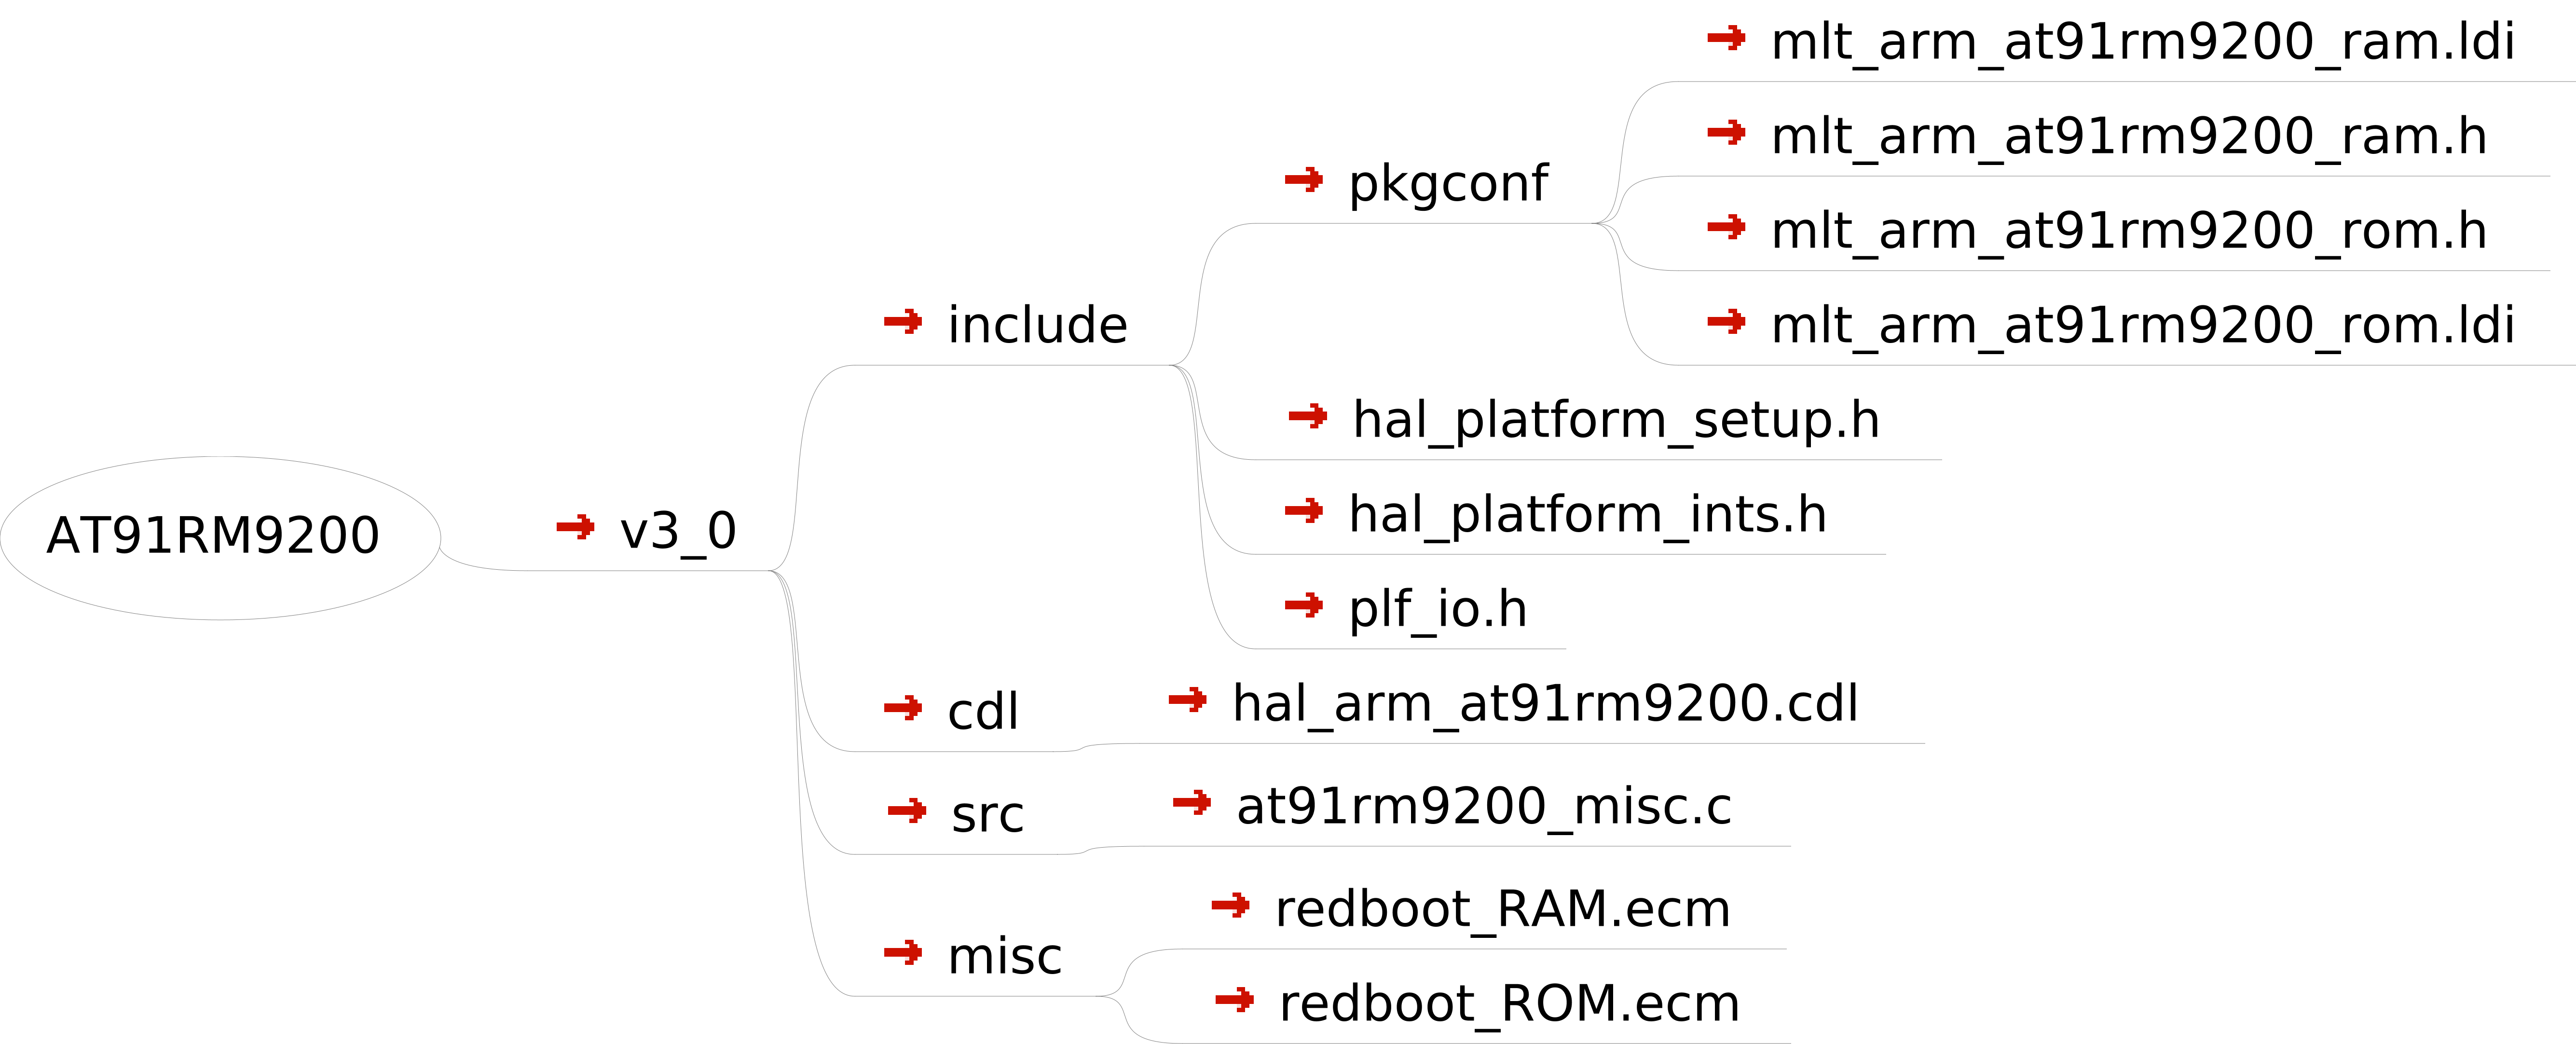
\includegraphics[width=12cm]{HAL_Dir_Map}
\caption{AT91RM9200 HAL Verzeichnisstruktur}
\label{fig:HAL_Dir_Map}
\end{figure}

Die Datei \texttt{hal\_arm\_at91rm9200.cdl} enthält die \emph{Paket-Beschreibung} für eCos. In dieser werden alle nötigen Referenzen auf den \emph{AT91SAM7} Prozessor durch neue ersetzt. Hierzu gehören zum Beispiel die zu verwendenden Linker-Skripte und Compiler-Anweisungen.

Der Ordner \texttt{./include/pkgconf} enthält die \emph{Linker-Skripte} sowohl für die Ausführung aus dem RAM als auch aus dem ROM. Im Rahmen dieser Arbeit wird lediglich die RAM-Variante näher betrachtet. Zusätzlich wird in eCos eine Header-Datei erstellt, die verschiedene Präprozessor-Anweisungen enthält.

\begin{lstlisting}[frame=single, float, caption={Linker-Skript RAM}, label={lst:linker_skript_ram}]
#include <cyg/infra/cyg_type.inc>
#include <pkgconf/hal_arm_at91rm9200.h>

MEMORY
{
    ram : ORIGIN = 0x20000000, LENGTH = 0x80000
    rom : ORIGIN = 0x10000000, LENGTH = 0x40000
}

SECTIONS
{
    SECTIONS_BEGIN
    . = 0x20000000;
    .vectors ALIGN (0x4) : { . = .; *(.vectors) } > ram
    SECTION_text (ram, ALIGN (0x1), LMA_EQ_VMA)

    [...]

    CYG_LABEL_DEFN(__heap1) = ALIGN (0x8);
    SECTIONS_END
}
\end{lstlisting}

Wie im Quellcode-Listing \ref{lst:linker_skript_ram} zu sehen ist, werden wie üblich im ersten Abschnitt die \emph{Speicherbereiche} definiert. In diesem Fall ein externer RAM und ROM. Im darunter liegenden Abschnitt werden die \emph{Segmente} im Speicher verteilt und einige \emph{Labels} definiert. Hierzu werden wie bei eCos üblich, Präprozessor Makros verwendet.

\begin{lstlisting}[frame=single, float, caption={Linker-Skript RAM Header}, label={lst:linker_skript_ram_header}]
#define CYGMEM_REGION_ram (0x20000000)
#define CYGMEM_REGION_ram_SIZE (0x80000)
#define CYGMEM_REGION_ram_ATTR (CYGMEM_REGION_ATTR_R | CYGMEM_REGION_ATTR_W)
[...]
\end{lstlisting}

Einen Eindruck vom Inhalt des Linker-Skript-Headers, gibt Code-Listing \ref{lst:linker_skript_ram_header}. In diesem werden Angaben zu den Speicherbereichen gemacht, die ähnlich auch im Linker Skript zu finden sind. So gibt die erste Zeile die Startadresse an und die zweite die Größe des RAM an.

Um eCos mitzuteilen wie die \emph{Interrupts} des Systems spezifiziert sind, existiert die Datei \texttt{hal\_platform\_ints.h}. Hierin werden den Interrupt-Bezeichnern die dazugehörigen IDs zugewiesen. Die Datei \texttt{plf\_io.h} enthält die Definition einiger Speicherbereiche von diverser Peripherie. Da die Peripherie sich jedoch bei den verschiedenen Prozessor-Modellen ähnelt, werden die meisten Bereiche im Variant-HAL definiert. Dies ist im nächsten Kapitel zu finden. Ausschnitte aus den Dateien \texttt{hal\_platform\_ints.h} und \texttt{plf\_io.h} sind in Quellcode-Listing \ref{lst:ints_plf_io} zu finden.

\begin{lstlisting}[frame=single, float, caption={hal\_platform\_ints.h und plf\_io.h}, label={lst:ints_plf_io}]
hal_platform_ints.h:
  #define CYGNUM_HAL_INTERRUPT_PIOA   2
  #define CYGNUM_HAL_INTERRUPT_IRQ6   31

plf_io.h:
  #define AT91_PIOA      0xFFFFF400
  #define AT91_PIOB      0xFFFFF600
\end{lstlisting}

Der Quellcode um die Hardware zu initialisieren ist in der Datei \texttt{hal"-\_"-plat"-form"-\_"-set"-up.h} enthalten. Da das Projekt jedoch aus dem RAM läuft, und so die \emph{Initialisierung} vom OpenOCD übernommen wird, ist die Datei relativ leer. Wie in Listing \ref{lst:hal_setup} zu sehen ist, wird ein Makro definiert, das den Code enthält. In diesem Fall ist dieser Abschnitt jedoch leer. Von eCos wird das Makro über den Aufruf von \texttt{PLATFORM\_SETUP1} gestartet. 

\begin{lstlisting}[frame=single, float, caption={hal\_platform\_setup.h}, label={lst:hal_setup}]
        .macro  _setup
__setup:
	[...]
        .endm
#define PLATFORM_SETUP1     _setup
\end{lstlisting}

Zusätzlich enthält der HAL die C-Datei \texttt{at91rm9200\_misc.c}, in der zwei grundlegende Funktionen definiert sind (Siehe Listing \ref{lst:at91rm9200_misc}). Die erste Funktion enthält weitere \emph{Hardware-Initialisierungen} und verwendet eCos Makros, um die Pins zu konfigurieren. Die zweite Funktion berechnet den Wert für das \emph{Baud-Rate-Register} der \emph{seriellen Schnittstelle}.

\begin{lstlisting}[frame=single, float, caption={at91rm9200\_misc.c}, label={lst:at91rm9200_misc}]
void hal_plf_hardware_init (void) {
  HAL_ARM_AT91_PIO_CFG(AT91_USART_RXD2);
  HAL_ARM_AT91_PIO_CFG(AT91_USART_TXD2);
  [...]
}

cyg_uint32 hal_at91_us_baud(cyg_uint32 baud_rate) {
  [..]
  return baud;
}
\end{lstlisting}

\begin{figure}
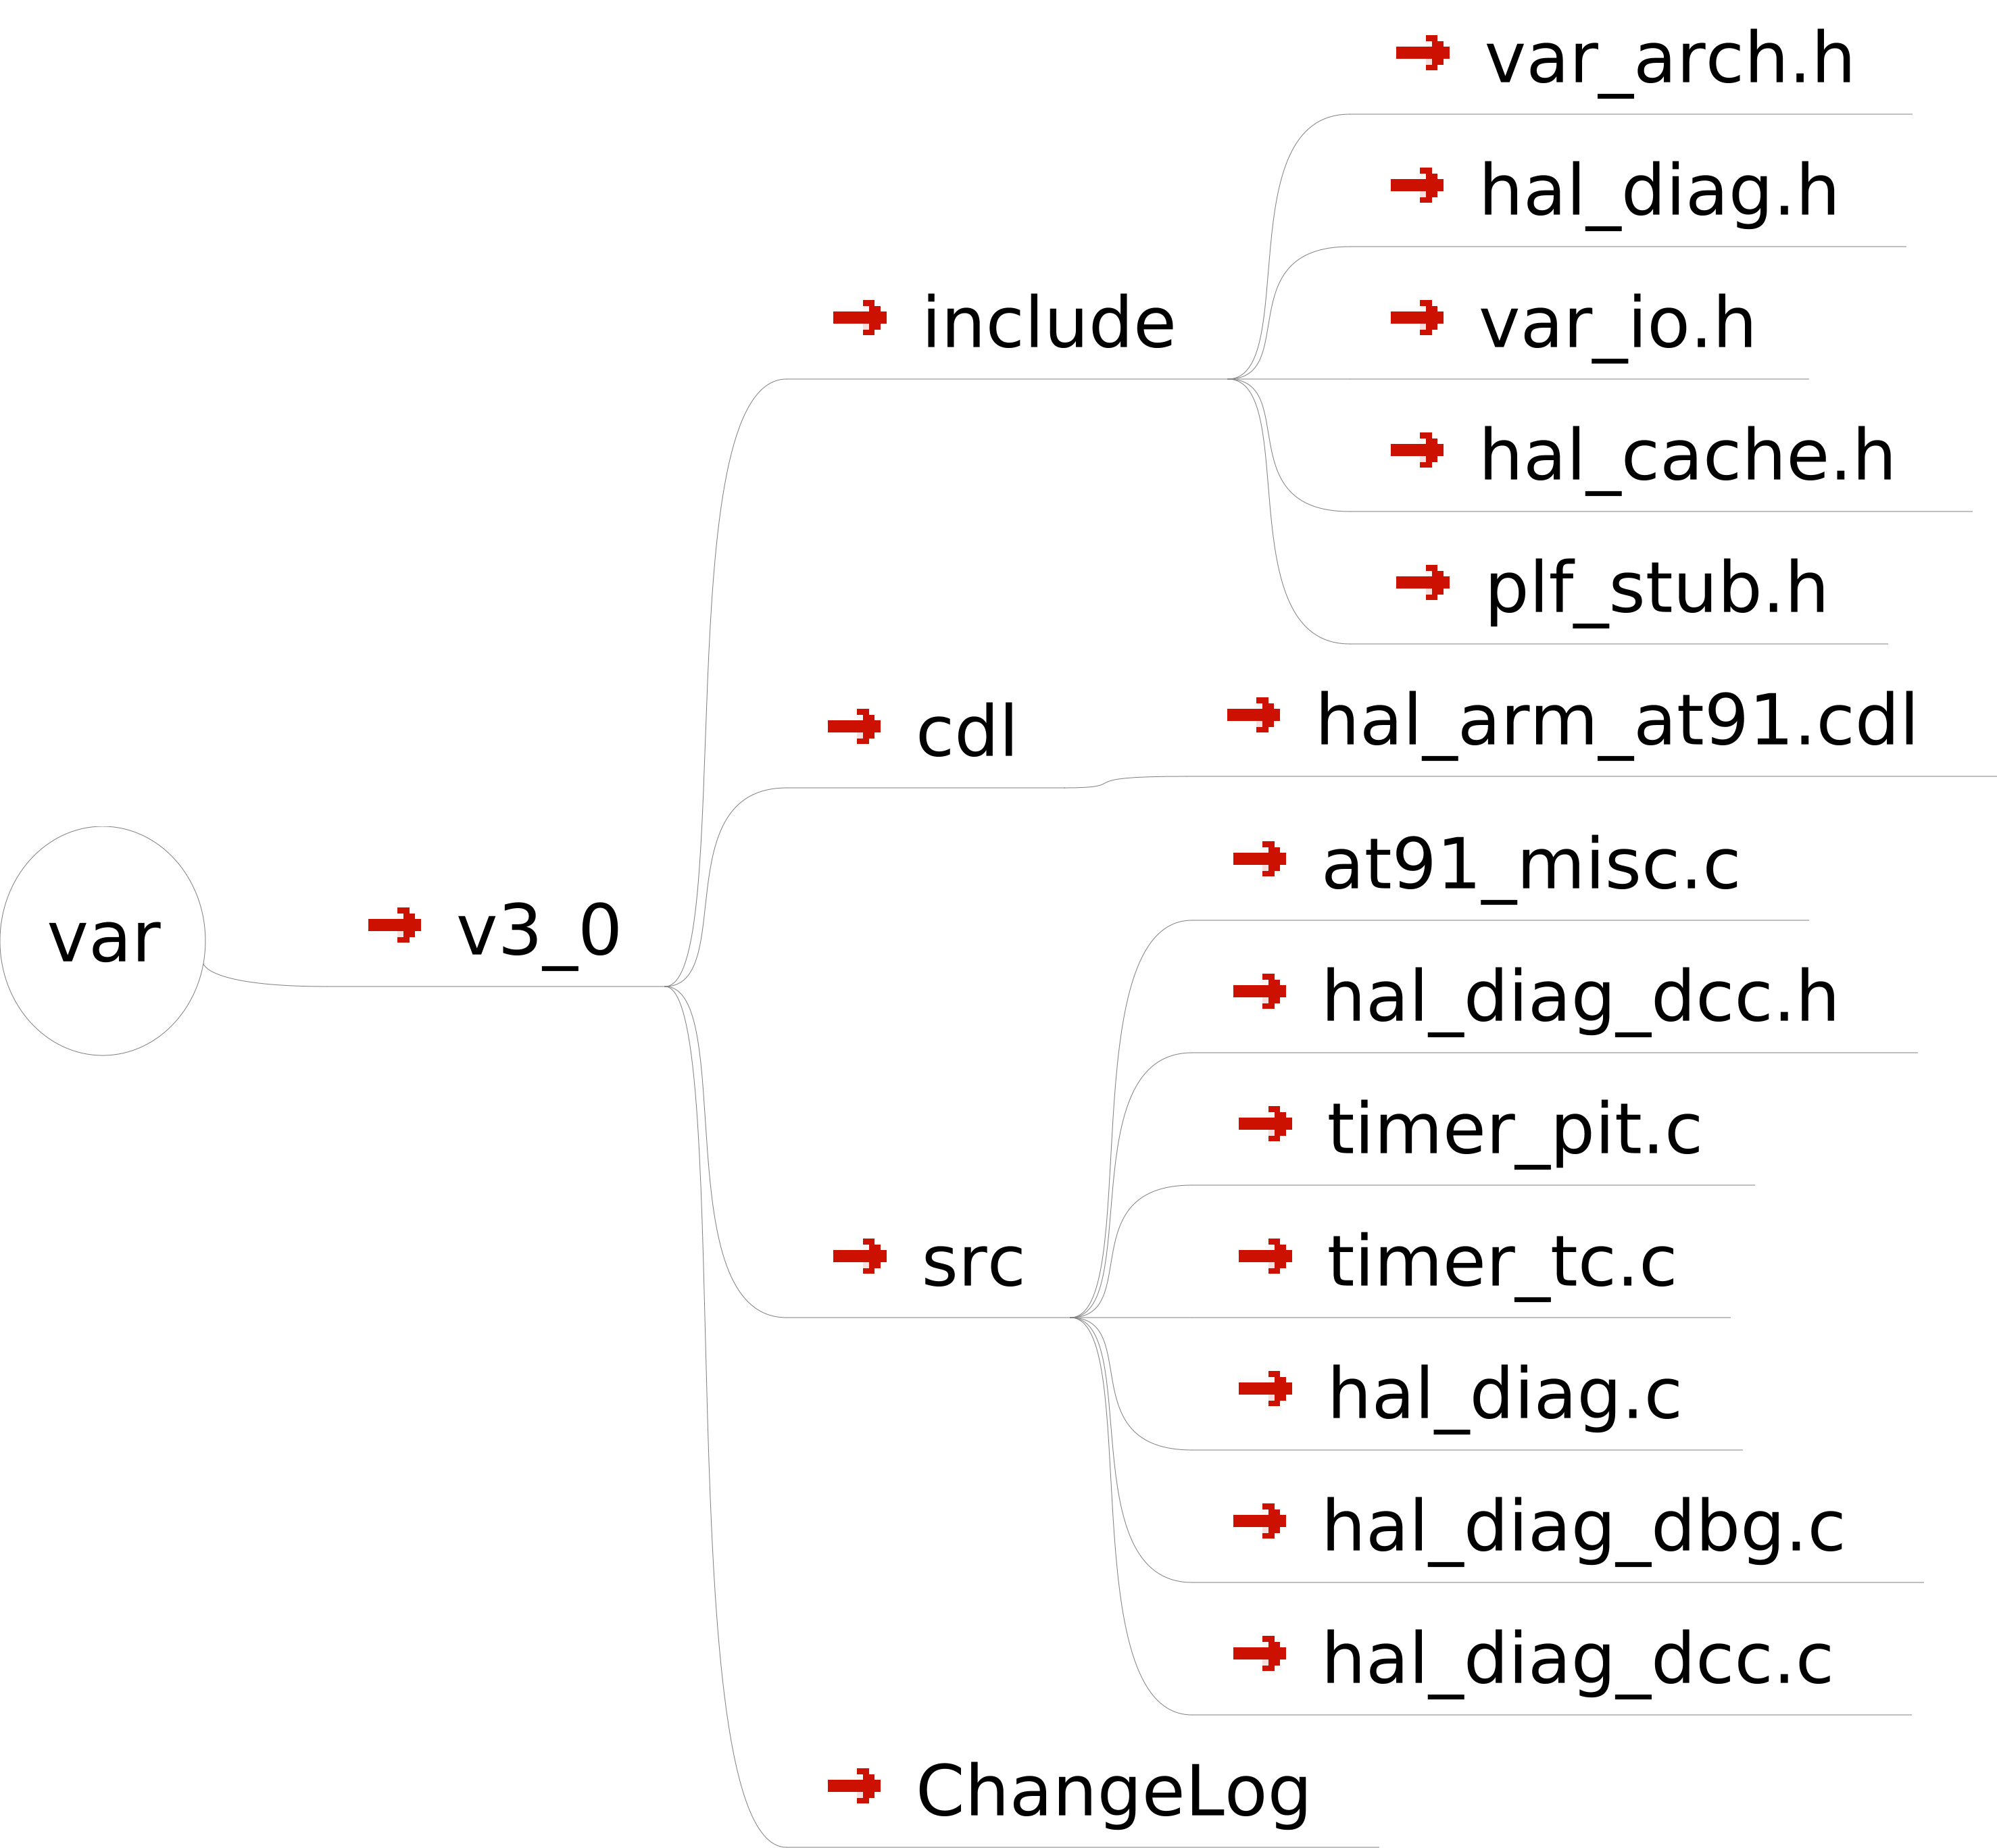
\includegraphics[width=6cm]{HAL_Var_Dir_Map}
\caption{Variant HAL Verzeichnisstruktur}
\label{fig:HAL_Var_Dir_Map}
\end{figure}

Neben diesem prozessorspezifischen Teil des HALs, existiert im Verzeichnis \texttt{./hal/arm/at91/var} zudem eine Reihe von Dateien, die von allen Prozessoren der AT91 Serie genutzt werden. Die hierin verwendete Datei-Struktur ist in Abbildung \ref{fig:HAL_Var_Dir_Map} zu sehen. Viele der Dateien sind nicht weiter relevant und werden nicht genauer erläutert.

Die Hardware-Beschreibung, die bereits zum Teil in der Datei \texttt{plf\_io.h} stattfindet, wird in dem Header \texttt{var\_io.h} weitergeführt. Diese Trennung wurde eingeführt, um einzelne Register innerhalb der Plattform-Beschreibung zu überschreiben. Neben den Speicher-Adressen der Register, werden in dieser Datei auch Werte dieser Register und das Pin-Out des Prozessor beschrieben. Beispiele hierzu sind im Quellcode-Listing \ref{lst:var_io} zu finden.

\begin{lstlisting}[frame=single, float, caption={var\_io.h}, label={lst:var_io}]
#define AT91_US_CR_RxRESET   (1<<2)
#define AT91_USART_RXD0      AT91_PIN(0,0,22)
[...]
\end{lstlisting}

Einen weiteren Teil der Hardware-Initialisierung enthält die Datei at91\_misc.c. Zudem ist hier einiger Code für die \emph{Interrupt-Behandlung} untergebracht. Zum Beispiel das Dekodieren des System-Interrupts.

Um einfache Ausgaben über die serielle Schnittstelle zu erlauben, ist in der Datei \texttt{hal\_diag.c} ein einfacher, per Polling implementierter, Treiber zu finden. Über diesen kann sowohl RedBoot, als auch eCos System-Ausgaben machen. Auch zum Debuggen des Codes ist dieser sehr hilfreich.

In der Datei \texttt{timer\_tc.c} sind alle Funktionen enthalten, die gebraucht werden, um die von eCos benötigten Clocks zu verwenden. Da der AT91RM9200 eine andere \emph{PIT-Implementation} enthält als der AT91SAM7, wird zunächst ein \emph{Timer} als System-Clock verwendet. In einem späteren Kapitel wird diese auf den PIT geändert.

Da alle ARM-Prozessoren sich in einigen Teilen gleichen, existiert im Verzeichnis \texttt{./hal/arm/arch} ein weiterer Abschnitt des HAL. Die meisten Dateien definieren hier neue Funktionen oder Präprozessor-Makros. Da diese jedoch nicht weiter bearbeitet wurden, werden sie auch hier nicht weiter betrachtet. Lediglich die Dateien \texttt{arm.ld} und \texttt{vectors.S} sollen hier kurz vorgestellt werden. Die Datei \texttt{context.S}, die für den \emph{Kontext-Wechsel} bei Thread-Wechseln verwendet wird, wird außerdem in einem späteren Kapitel näher betrachtet.

Hinter der Datei \texttt{arm.ld} versteckt sich das \emph{Linker-Skript}. Obwohl zu Beginn dieses Kapitels bereits ein Linker-Skript vorgestellt wurde, ist dies die eigentliche Datei. Hier werden alle Makros definiert, die im anderen Skript verwendet werden. Ein Ausschnitt aus der Datei \texttt{arm.ld} findet sich in Listing \ref{lst:arm_ld}. Wie dort zu sehen ist, wird zu Beginn des Skripts die Datei \texttt{vectors.o} und das Label \texttt{reset\_vector} als Einstiegspunkt definiert. Anschließend werden einige Makros definiert. In diesem Beispiel für das Segment \texttt{fixed\_vectors}. Die letzte Zeile des Skripts bindet das zu Beginn des Kapitels vorgestellte Linker-Skript ein. Dies geschieht über eine Präprozessor Variable, die mittels des Configtools gesetzt wird.

\begin{lstlisting}[frame=single, float, caption={arm.ld}, label={lst:arm_ld}]
STARTUP(vectors.o)
ENTRY(reset_vector)
[...]
#define SECTION_fixed_vectors(_region_, _vma_, _lma_) \
    .fixed_vectors _vma_ : _lma_ \
    { FORCE_OUTPUT; KEEP (*(.fixed_vectors)) } \
    > _region_
[...]
#include CYGHWR_MEMORY_LAYOUT_LDI
\end{lstlisting}

Die Datei \texttt{vectors.S} enthält die \emph{Interrupt-Vektor-Tabelle} und die grundlegende Initialisierung. Einige Ausschnitte finden sich in Listing \ref{lst:vectors}. Da eCos eine Reihe von Konfigurations-Möglichkeiten bietet, werden diese Fälle durch Präprozessor-Anweisungen getrennt. Dies führt dazu, dass der Quellcode relativ schwer zu lesen ist. Aus diesem Grund werden im Auszug lediglich drei wichtige Abschnitte gezeigt. Im ersten Teil wird die Interrupt-Vektor-Tabelle zusammengestellt. Hier wird zum Beispiel überprüft, ob bei der Ausführung aus dem ROM ein Sprung (Branch) benutzt werden soll oder nicht. Im zweiten Abschnitt wird das \emph{Label} \texttt{reset\_vector} definiert, dass als Einstiegspunkt fungiert. Hier wird zunächst der Hardware-Initialisierungs-Code aufgerufen. Anschließend wird zum Beispiel das \texttt{bss}-Segment auf null initialisiert. Zu Letzt wird ein Sprung ins eigentliche Betriebssystem ausgeführt. Ab hier übernimmt je nach Konfiguration \emph{eCos} oder \emph{Reboot}. Für den Fall das mittels \texttt{return} an diese Stelle zurückgesprungen wird, ist eine Endlosschleife implementiert.

\begin{lstlisting}[frame=single, float, caption={vectors.S}, label={lst:vectors}]
#ifdef CYGSEM_HAL_ROM_RESET_USES_JUMP
        b       reset_vector                    // 0x00
#else        
        ldr     pc,.reset_vector                // 0x00
#endif        
        ldr     pc,.undefined_instruction       // 0x04
        ldr     pc,.software_interrupt          // 0x08
        ldr     pc,.abort_prefetch              // 0x0C
        ldr     pc,.abort_data                  // 0x10
#ifdef CYGNUM_HAL_ARM_VECTOR_0x14
        .word   CYGNUM_HAL_ARM_VECTOR_0x14
#else
        .word   0                               // unused
#endif
        ldr     pc,.IRQ                         // 0x18
        ldr     pc,.FIQ                         // 0x1C
[...]
reset_vector:
        PLATFORM_SETUP1 
[...]
        bl      cyg_start
\end{lstlisting}

Der letzte Teil des Hardware-Abstraction-Layers ist der \emph{Common-Hal} und befindet sich im Verzeichnis \texttt{./hal/common}. Dieser enthält Code der von allen HAL-Paketen genutzt wird. Die hierin enthaltenen Dateien sollen nicht weiter erläutert werden, da diese nicht verändert wurden.

Neben dem AT91RM9200 HAL wird noch ein zusätzliches Paket für den UNC90 Plattform HAL erstellt. Da dieses Paket zur Zeit keinen relevanten Inhalt hat, wird es auch nicht weiter erläutert. Jedoch kann dieses Paket für zukünftige Änderungen an plattform-bedingten Komponenten, wie Tastern oder ähnlichem, benutzt werden.

Um die erstellten Pakete nun verwenden zu können, müssen noch entsprechende Einträge in der eCos-Paket-Datenbank gemacht werden. Und um den Zugriff hierauf zu vereinfachen, wird zusätzlich eine Vorlage definiert. Ein Auszug aus den Änderungen der Datei \texttt{ecos.db} ist in Listing \ref{lst:ecos_db} zu sehen.

\begin{lstlisting}[frame=single, float, caption={ecos.db}, label={lst:ecos_db}]
package CYGPKG_HAL_ARM_AT91RM9200 {
	alias		{ "Atmel AT91RM9200" hal_arm_at91rm9200 arm_at91_rm9200 }
	directory	hal/arm/at91/at91rm9200
	script		hal_arm_at91rm9200.cdl
	hardware
        description "
	Test Port for Atmel AT91RM9200"
}
[...]
target unc90 {
	alias { "Digi UNC90" at91_unc90 }
	packages { CYGPKG_HAL_ARM
                   CYGPKG_HAL_ARM_AT91
                   CYGPKG_HAL_ARM_AT91RM9200
                   CYGPKG_HAL_ARM_UNC90
        }
        description "
        Test Port for Digi UNC90 with Atmel AT91RM9200"
}
\end{lstlisting}





% Configtool einstellungen; redboot template
% USART einrichten / reparieren
% Baud-Rate, const zu Tabelle in hal_diag.c hinzugefügt
\section{Serielle Schnittstelle}
\label{sec:USART}

Nachdem nun die Grundlage, der HAL, geschaffen ist, wird nun mit Hilfe des Configtools eine erste Konfiguration erstellt. Hierzu wird über das Menü \texttt{Build->Templates} die vorher erstelle Vorlage ausgewählt. In diesem Dialog-Fenster ist es auch möglich verschiedene Paket-Zusammenstellungen auszuwählen. Laut eCos Referenz ist es dabei von Vorteil, das Profil \emph{redboot} zu verwenden. Dies beinhaltet lediglich die verschiedenen \emph{HAL-Pakete}, das \emph{Infrastructure} Paket, das \emph{RedBoot} Paket und drei Pakete zur \emph{Unterstützung} von zum Beispiel Strings und ähnlichem.

Um nun ein Projekt zu kompilieren, wird die \emph{Konfiguration} im Configtool gespeichert. Dabei wird gleichzeitig der Install- und Build-Tree errichtet. Innerhalb des Build-Trees befindet sich ein \emph{Makefile}, das bei der Ausführung den Quellcode kompiliert, und das Ergebnis im Build-Tree abspeichert. Diese \emph{Binary} kann nun mittels der bereits beschriebenen Weise auf die Ziel-Plattform gespielt werden. Der bisher entstandene Port und die Konfiguration sind jedoch noch nicht komplett lauffähig.

Der nächste wichtige Schritt ist das Einrichten der \emph{seriellen Schnittstelle}. Für den Fall das beim Erstellen des HAL bereits alle Pins und Register korrekt eingerichtet wurden, ist nun lediglich das Konfigurieren des USART im Configtool nötig. 

Während meiner Arbeit kam es anschließend zu keiner Ausgabe auf der Konsole. Nach einigem Suchen konnte ich feststellen das ein Fehler in der Initialisierung der seriellen Schnittstelle im Variant-HAL auftritt. Hier werden die Daten aller im System vorhandener seriellen Schnittstellen in einem Array gespeichert. Dieses Array wurde zwar prinzipiell korrekt initialisiert, jedoch später mit falschen Werten verändert. Hierdurch kam es zu falschen Basis-Adressen der Schnittstellen. Dieser Fehler konnte durch das einfache Hinzufügen des Schlüsselwortes \texttt{const} behoben werden. Somit kann das Array nicht mehr verändert werden und die Basis-Adressen liegen korrekt vor. 

% Baud-Rate im src ändern?
Nach dieser Änderung wurden erste Zeichen auf der seriellen Schnittstelle ausgegeben. Da diese jedoch nicht zu entziffern waren, fiel der Verdacht auf die Funktion zum Generieren der Baud-Rate. Da diese von einigen Faktoren abhängt und relativ Fehleranfällig zu sein scheint, wurde der dynamisch berechnete Wert durch einen statischen ersetzt. Da die Konfiguration der Baud-Rate indirekt mit dem Prozessor-Takt zusammenhängt, kommt es jedoch beim Ändern von diesem zu einer fehlerhaften Baud-Rate. 

% Redboot einrichten
% Linker-Skript Fehler
% Aus RAM starten
\section{Redboot}
\label{sec:Reboot}

Obwohl nun die serielle Schnittstelle funktioniert, und auch RedBoot startet, können in der RedBoot-Shell keine Befehle ausgeführt werden. Sobald ein Kommando ausgeführt werden soll, wird stattdessen an einen falschen \emph{Speicherbereich} gesprungen. Nach einigem Suchen stellte sich heraus, das die Liste in der die Kommandos gespeichert werden, zwar in der Binary im richtigen Bereich liegen, jedoch nach dem Übertragen in den Speicher nicht mehr so vorhanden sind. Beim genaueren Untersuchen des \emph{Linker-Skripts} stellte sich heraus, dass das \texttt{data}-Segment mit der Option \texttt{following} eingefügt wurde. Dies führt dazu, dass dies Segment im Speicher immer einem bestimmten anderen folgt. Durch das Mischen der eCos Syntax und der Linker-Syntax führte dies dazu, dass Teile des Speichers mehrmals beschrieben wurden, und so die Kommando-Tabelle überschrieben wurde. Nachdem der \texttt{following} Befehl entfernt wurde, und das Segment mit den üblichen Eigenschaften eingefügt wurde, kam es innerhalb von RedBoot zu keinen Fehlern mehr.

Zu diesem Zeitpunkt laufen nun die Grundlegenden Funktionen des HAL, und RedBoot kann als Bootloader verwendet werden. Jedoch existiert noch keine \emph{Stand-Alone eCos Applikation}. Dies wird im nächsten Kapitel beschrieben. RedBoot kann jedoch auch Debug-Funktionen bereitstellen. Zu diesem Zweck besitzt eCos das sogenannte \emph{ROM Monitor Calling Interface}, dass durch die Virtuellen Vektoren realisiert ist. Da die Debug-Funktionen von RedBoot in diesem Projekt nicht weiter benötigt werden, wurde dies auch nicht weiter getestet.



% eCos Kernel compilieren
\section{eCos Kernel}
\label{sec:eCos_Kernel}
Um eine \emph{eCos-Binary} zu erzeugen, muss mittels des Configtools eine neue Konfiguration erstellt werden, die die entsprechende Kernel-Pakete enthält. Hierzu kann wie schon vorher beschrieben eine Paket-Zusammenstellung verwendet werden. Im weiteren wird, wenn nicht anders genannt, die \emph{Default} Paket-Vorlage verwendet. Diese enthält alle \emph{HAL-Pakete}, das \emph{Infrastructure} Paket, den \emph{eCos Kernel} und einige \emph{Unterstützungs-Pakete}, wie die Math-Library oder die ISO-C-Library.

Der darauf folgende Ablauf entspricht dem von RedBoot. Beim Kompilieren wird jedoch keine direkt ausführbare Datei erzeugt. Stattdessen wird eine \emph{Library} erzeugt. Neben dieser ist im Install-Tree außerdem ein \emph{Linker-Skript} und alle nötigen \emph{Header-Dateien} vorhanden. Mit Hilfe dieser Elemente kann die eigene Software kompiliert und gegen den eCos-Kernel gelinkt werden. Dabei werden während des Link-Prozesses alle unnötigen Funktionen entfernt, sodass die Ausgabe-Datei eine minimale Größe besitzt. Der dazu nötige \emph{Compiler-Aufruf}\cite{gcc_manual} ist in Listing \ref{lst:compiler_aufruf} zu sehen. Mittels der Option \texttt{-g} wird das generieren von \emph{Debug-Informationen} für den gdb aktiviert. Dies ist nicht zwingend erforderlich. Um die \emph{Header-Dateien} und die \emph{eCos Library} zu verwenden, werden die Optionen \texttt{-I} und \texttt{-L} eingefügt. Mittels der Option \texttt{-T} wird das \emph{Linker-Skript} definiert, und der Befehl \texttt{-nostdlib} gibt an das nur die per Paramter übergebenen Librarys, Header und das Linker-Skript verwendet werden sollen.

\begin{lstlisting}[frame=single, float, caption={Compiler-Aufruf}, label={lst:compiler_aufruf}]
arm-elf-gcc -g -I./install_tree/include target.c -L./install_tree/lib -Ttarget.ld -nostdlib
\end{lstlisting}





% App gegen Kernel kompilieren
% Hello World lief
% Thread macht Fehler: movs zu mov in context.S
% eCos Thread wird nur einmal ausgeführt
% POSIX Threads brechen bei sleep Funktion ab.
\section{Beispiel Applikation}
\label{sec:BeispielApp}
Nachdem die Grundlagen nun erläutert wurden, kann nun die erste Applikation getestet werden. Hierzu kann eine einfache C-Datei geschrieben werden, in der die Funktion \texttt{cyg\_user\_start()} die \texttt{main()}-Funktion ersetzt. Für den ersten Test habe ich ein simples \emph{Hello-World} verwendet (siehe Listing \ref{lst:hello_world}). Nachdem dieses gegen den Kernel kompiliert und auf die Plattform geladen wurde, konnte es erfolgreich ausgeführt werden.

\begin{lstlisting}[frame=single, float, caption={Hello World}, label={lst:hello_world}]
void cyg_user_start(void) {
  printf("Hello World\n");
}
\end{lstlisting}

Nächstes Programm ist ein Test des \emph{eCos-Thread-Systems}. Hierzu werden zwei einfach Threads erstellt die jeweils eine Ausgabe auf der Konsole machen. Der dazugehörige Quellcode ist in Listing \ref{lst:ecos_threads} zu finden. Beim Testen dieses Beispiels kam es zu einem unerwünschten Effekt. Beim \emph{Thread-Kontext-Wechsel}, wurde das PC-Register auf eine falsche Speicher-Adresse gesetzt. Nach genauerem Suchen konnte ich das Problem auf eine Funktion, genauer einen Befehl in dieser zurückführen. In diesem wird das LR-Register ins PC-Register geschrieben. Im Original-Code wird dies mittels des \texttt{movs}-Befehls erledigt. Sobald dieser Befehl jedoch mittels des Debuggers von Hand emuliert wird, lief der Thread-Wechsel ohne Probleme durch. Somit wurde der Befehl \texttt{movs} durch einen einfachen \texttt{mov}-Befehl ersetzt. Nach dieser Änderung wurden beide Threads nacheinander ausgeführt. 

Bei späterer genauerer Betrachtung zeigte sich jedoch, dass die kleine Änderung zu einem schwerwiegenden Fehler führt. Im Gegensatz zu dem einfachen \texttt{mov}-Befehl, wird der \texttt{movs}-Befehl verwendet um gleichzeitig ein Register zu schreiben und das \emph{Status-Register} zu aktualisieren. Somit führt also diese Änderung zu einem Verlust der Status-Register beim Kontext-Wechsel. Zu einem späteren Zeitpunkt konnte dieser Änderung ohne Folgen rückgängig gemacht werden. Wahrscheinlich führten aktivierte Interrupts zuvor zu dem unvorhersehbaren Verhalten.

Nach dieser Änderung wurde der Quellcode leicht verändert, sodass die Konsolen-Ausgabe zyklisch erfolgt. Beim Ausführen dieses Projekts, fiel auf, dass jeder Thread nur einmal ausgeführt wird. Hierbei fiel mein Verdacht auf den verwendeten \emph{Timer}. Dies Problem wurde jedoch vorerst nicht weiter betrachtet.

\begin{lstlisting}[frame=single, float, caption={eCos Threads}, label={lst:ecos_threads}]
cyg_thread thread_s[2];
char stack[2][4096];
cyg_handle_t simple_threadA, simple_threadB;
cyg_thread_entry_t simple_program;
cyg_mutex_t cliblock;

void cyg_user_start(void)
{
  printf("Entering cyg_user_start()\n");
  cyg_mutex_init(&cliblock);
  cyg_thread_create(4, simple_program, 0, "Thread A", (void *) stack[0], 4096, &simple_threadA, &thread_s[0]);
  cyg_thread_create(4, simple_program, 0, "Thread B", (void *) stack[1], 4096, &simple_threadB, &thread_s[1]);
  cyg_thread_resume(simple_threadA);
  cyg_thread_resume(simple_threadB);
}

void simple_programA(cyg_addrword_t data)
{
  while (true) {
    cyg_mutex_lock(&cliblock); {
      printf("A"); }
    cyg_mutex_unlock(&cliblock);
    cyg_thread_delay(100);
  }
}

void simple_programB(cyg_addrword_t data)
{
  while (true) {
    cyg_mutex_lock(&cliblock); {
      printf("B"); }
    cyg_mutex_unlock(&cliblock);
    cyg_thread_delay(100);
  }
}
\end{lstlisting}

Um die \emph{POSIX-Kompatibilität} zu testen, wird das vorherige Beispiel übernommen und mit der POSIX-API implementiert. Der hierzu gehörige Quellcode befindet sich in Listing \ref{lst:posix_threads}. Da die \emph{Default}-Vorlage keine volle POSIX-Unterstützung bietet, wird das entsprechende Paket von Hand hinzugefügt. 

\begin{lstlisting}[frame=single, float, caption={POSIX Threads}, label={lst:posix_threads}]
#include <pthread.h>

void *TaskCodeA()
{
  while (true) {
    printf("A\n");
  }
}

void *TaskCodeB()
{
  while (true) {
    printf("B\n");
  }
}

void cyg_user_start(void) {
	pthread_t thread_contextA;
	int rcA;
	pthread_attr_t use_attrA;
	pthread_t thread_contextB;
	int rcB;
	pthread_attr_t use_attrB;
	pthread_attr_init( &use_attrA );
	pthread_attr_init( &use_attrB );

	rcA = pthread_create(&thread_contextA, &use_attrA, TaskCodeA, NULL);
	rcB = pthread_create(&thread_contextB, &use_attrB, TaskCodeB, NULL);

	rcA = pthread_join(thread_contextA, 0);
	rcB = pthread_join(thread_contextB, 0);

	pthread_exit(NULL);
}
\end{lstlisting}

Auch dieses Projekt lief nicht ohne Probleme auf der Hardware. Hierbei kam es bei den \texttt{sleep}- und \texttt{delay}-Funktionen zu Problemen, sodass einmal schlafende Threads nicht mehr aufgeweckt wurden. Wieder einmal fiel der Verdacht auf den verwendeten \emph{Timer}. 




% Einrichten für den Scheduler
% TC durch PIT ersetzen
% Interrupt richten
\section{Timer}
\label{sec:Timer}

Da der AT91RM9200 eine andere Implementation eines \emph{Periodic-Interval-Timer}, kurz PIT, besitzt, wurde zu Beginn des Projekts die Systemclock mit Hilfe eines einfachen \emph{Timers} realisiert. Da diese jedoch auch für andere Zwecke genutzt werden, ist es Sinnvoll die \emph{Systemclock} durch den PIT zu realisieren. Hierzu muss lediglich innerhalb der Konfiguration eine Option verändert werden und in der Datei \texttt{./hal/arm/at91/var/src/timer\_pit.c} die Implementation angepasst werden. Um Kompatibilität zu gewährleisten, wird eine Option hinzugefügt mit der die AT91RM9200-Implementation des PIT eingeschaltet wird. Ein Auszug aus dem Quellcode ist in Listing \ref{lst:pit_code} zu finden.

\begin{lstlisting}[frame=single, float, caption={PIT Implementation}, label={lst:pit_code}]
void hal_clock_initialize(cyg_uint32 period) {

#ifdef CYGBLD_HAL_ARM_AT91_TIMER_PIT_RM9200

  /* Set Period Interval Value */
  HAL_WRITE_UINT32((AT91_ST + AT91_ST_PIMR), period);

  /* Enable Interrupt */
  cyg_uint32 imr;
  HAL_READ_UINT32((AT91_ST + AT91_ST_IMR), imr);
  HAL_WRITE_UINT32((AT91_ST + AT91_ST_IER), (imr | 0x1));

#else

[...]

#endif
}
\end{lstlisting}

Nach dieser Veränderung ist der PIT korrekt eingerichtet. Um die \texttt{delay}-Funktion und ähnliches zu unterstützen, muss dieser jedoch auch einen Interrupt auslösen. Hierzu werden im PIT und im AIC die entsprechenden Register gesetzt, um den Interrupt freizuschalten. 

Nun ist der Interrupt zwar korrekt eingerichtet, jedoch besteht immer noch ein Problem durch einen Fehler im Linker-Skript. Die \emph{Interrupt-Vektor-Tabelle} wird vom Prozessor an Adresse Null erwartet. Laut Linker-Skript liegt diese jedoch am Anfang des externen RAMs (Adresse 0x20000000). Dies lässt sich durch das Einführen eines weiteren Speicher-Bereichs im Linker-Skript erreichen. Ein Auszug des verbesserten Linker-Skripts ist in Quellcode-Listing \ref{lst:linker_skript_fixed} zu finden.

\begin{lstlisting}[frame=single, float, caption={Verbesserters Linker-Skript}, label={lst:linker_skript_fixed}]
MEMORY
{
    ram : ORIGIN = 0x20000000, LENGTH = 0x80000
   boot : ORIGIN = 0x00000000, LENGTH = 0x04000
}

SECTIONS
{
  [...]
  .vectors ALIGN (0x4) : { . = .; *(.vectors) } > boot
  . = 0x20000000;
  SECTION_text (ram, ALIGN (0x4), LMA_EQ_VMA)
  [...]
}
\end{lstlisting}

Nach dieser letzten Änderung, können alle vorher erwähnten Test-Programme erfolgreich ausgeführt werden. Hiermit ist die rudimentäre Portierung erfolgreich.




\section{Erstellen des Patch}
\label{sec:Patch}
Um den veränderten Quellcode einfach verteilen zu können wird nun ein \emph{Patch} erstellt. Ein Patch ist ein inkrementelles Update für den Quellcode. Dieser kann mit Hilfe der Tools \texttt{diff} und \texttt{patch}, erstellt und ausgeführt werden. Listing \ref{lst:diff_patch} zeigt die beiden dazu nötigen Befehle. Der erste Befehl wird verwendet, um zwei Ordner miteinander zu vergleichen und das Ergebnis als Patch zu speichern. Die Kommandozeile-Schalter werden verwendet, um Leere Zeilen zu ignorieren, neue Dateien im Patch zu beachten und die Verzeichnisse rekursiv durchzugehen. Die zweite Zeile wendet nun den vorher erstellten Patch im aktuellen Verzeichnis an. Wichtig ist hierbei, dass ein Patch immer für eine bestimmte Version erstellt wird. Das bedeutet das nach Änderungen des Quellcodes, der Patch eventuell nicht mehr funktioniert. Das Ausführen des Patches kann mit der Option \texttt{--dry-run} simuliert und getestet werden.

\begin{lstlisting}[frame=single, float, caption={Diff und Patch Befehle}, label={lst:diff_patch}]
diff -BNr ./ecos_original/ ./ecos_port >> test.patch
patch [--dry-run] -i test.patch
\end{lstlisting}

Auf der beigelegten CD befinden sich zwei dieser Patch-Dateien. Diese fügen jeweils der Version 3 oder der aktuellen CVS Version von eCos den AT91RM9200 Port hinzu.

Um den Port dem offiziellen Repository hinzuzufügen, wurde am 25. Januar ein Ticket im Bug Management System von eCos erstellt. Dies ist die übliche Vorgehensweise beim Hinzufügen solcher Patches. Das Ticket trägt die Nummer 1001129 und wird hoffentlich endgültig in das CVS Repository übernommen.







%%%%%%%%%%%%%%%%%%%%%%%%%%%%%%% Projektmanagment %%%%%%%%%%%%%%%%%%%%%%%%%%%%%%%%%%
\chapter{Projektmanagment}
\label{sec:Projektmanagment}
% Projektmanagment
Das Projekt wurde, ähnlich dem Praxis-Projekt, nach einem \emph{iterativen Prinzip} durchgeführt. Hierzu wurde zuerst ein grober Prototyp entworfen, der später verbessert und erweitert wurde. Hierbei ist wichtig, dass nach jeder Neuerung der Prototyp möglichst lauffähig gemacht wird. Dies hat den Vorteil, dass während der Entwicklungsphase bereits ein \emph{Testbarer Prototyp} vorhanden ist. Das bedeutet auch, dass später in der Entwicklungsphase nützliche Hilfsmittel zur Verfügung stehen. So kann nach Einrichten der seriellen Schnittstelle die \texttt{printf}-Routine für Debug-Ausgaben genutzt werden. Auch die \emph{Assertions} (Überprüfen von Variablen während der Laufzeit) und das \emph{Tracing} (Auflistung von Funktionsaufrufen) von eCos sind eine Hilfe.








%%%%%%%%%%%%%%%%%%%%%%%%%%%%%%% Zusammenfassung %%%%%%%%%%%%%%%%%%%%%%%%%%%%%%%%%%
\chapter{Fazit und Ausblick}
\label{sec:FazitAusblick}
Während des Projekts konnten die Ziele in vollem Umfang erreicht werden. Es wurde ein rudimentärer HAL-Port erstellt, der als Grundlage für weitere Projekte dienen kann. Mit ein wenig Arbeit könnte dieser auch seinen Weg in die offizielle eCos Distribution finden.

Aufgrund der begrenzten Debug-Möglichkeiten, gab es im Projekt vor allem zu Beginn einige Schwierigkeiten. Nach und nach konnte der HAL jedoch verbessert und so das Debugging erleichtert werden. Das Projekt deckte einen weiten Themen-Bereich ab. Dieser reicht von der hardwarenahen Programmierung der Initialisierung bis hin zu abstrahierteren Schichten beim Implementieren des PIT.

Obwohl während dieses Projekts die Grundlage eines eCos-Port eingerichtet wurde, konnte bei weitem nicht die gesamte Hardware getestet werden. So könnte in einem zukünftigen Projekt die interne Hardware, wie der Cache, und die externe Hardware, wie Ethernet-Schnittstelle, eingerichtet werden. In diesem Zusammenhang kann auch die IPv6-Kompatibilität von eCos getestet werden.

Neben diesen Erweiterungen, könnte der bestehende eCos-Port durch die dazugehörigen Hardware-Tests genauer untersucht werden und bei Bedarf verbessert werden. Hierzu gehört auch das Trennen der Plattform und des Prozessor im HAL.




%%%%%%%%%%%%%%%%%%%%%%%%%%%%%%%%%%% Anhang %%%%%%%%%%%%%%%%%%%%%%%%%%%%%%%%%
\backmatter
\appendix
\part*{Anhang}






%%%%%%%%%%%%%%%%%%%%%%% Erklärung und CD %%%%%%%%%%%%%%%%%%%%%%%%%%%%%
\chapter{Erklärung}
\label{sec:Erklärung}
Hiermit erkläre ich, dass ich die vorliegende Arbeit selbstständig und nur unter Verwendung der angegebenen Quellen und Hilfsmittel erstellt habe.
\vspace{2.5cm} \par
Wolfenbüttel, den 10. Februar 2011


\chapter{Beigelegte CD}
\label{sec:BeigelegteCD}
Dieser Arbeit ist eine CD beigelegt, die die erstellten Materialien als auch die verwendete Software enthält. Folgende Daten wurde auf der CD abgelegt:

\begin{itemize}
  \item PDF-Version dieser Arbeit
  \item eCos Quellcode (Repository Version)
  \item eCos Quellcode inklusive Port
  \item Patch-Datei um eCos-Port zu bestehende Distribution hinzuzufügen
  \item OpenOCD Konfigurationsdatei
  \item OpenOCD Initialisierungs-Skript
  \item GNU-ARM Tool-Chain
  \item Datenblatt AT91RM9200
  \item Datenblatt UNC90
  \item Datenblatt UNCBAS3
\end{itemize}






%%%%%%%%%%%%%%%%%%%%%%%%%%%%%%% Bibliographie %%%%%%%%%%%%%%%%%%%%%%%%%%%%%%
% \setbibpreamble{Die Quellenangaben sind alphabetisch nach den Namen der Autoren sortiert.
% Bei mehreren Autoren wird nach dem ersten Autor sortiert.\par\bigskip\bigskip}
%
% Quellen, die nicht direkt zitiert wurden, aber trotzdem hier erscheinen sollen!
%\nocite{tbinformatik}\nocite{tb_et2000}\nocite{tb_mathe1999}
\nocite{*}
%
\begin{singlespace}
\bibliographystyle{natdin}		% alphadin, plaindin, abbrvdin, unsrtdin, natdin
					% germbib: gerabbrv, geralpha, gerplain, gerunsrt, gerapali, gerxampl
                           		% plainnat, abbrvnat, unsrtnat
                           		% Am besten geeignet: natdin
                           		% oder was ist mit dinat
                           		% ???apalike???
\bibliography{literature}
\end{singlespace}
%%%%%%%%%%%%%%%%%%%%%%%%%%%%%%%%%%%%%%%%%%%%%%%%%%%%%%%%%%%%%%%%%%%%%%%%%%%%

\end{document}


